% =====================================================================
%  Distributed SAT Solving with Dagster: virtual proceedings
%  decomposing an XOR session attack for strong scaling
%  Self-contained: all diagrams are TikZ, all plots are pgfplots with
%  the measured data embedded below.  Compile with pdflatex (twice).
% =====================================================================
\documentclass[11pt,a4paper]{article}

% Latin Modern with T1 encoding where installed; otherwise Computer Modern (Type 1)
\IfFileExists{lmodern.sty}{\usepackage[T1]{fontenc}\usepackage{lmodern}}{}
\usepackage[a4paper,margin=2.4cm]{geometry}
\usepackage{microtype}
\usepackage{amsmath,amssymb}
\usepackage{array,booktabs,longtable,multirow}
\usepackage{enumitem}
\usepackage{xcolor}
\usepackage{caption}
\usepackage{subcaption}
\usepackage[section]{placeins}
\renewcommand{\topfraction}{0.9}\renewcommand{\bottomfraction}{0.8}\renewcommand{\textfraction}{0.07}\renewcommand{\floatpagefraction}{0.75}
\setcounter{topnumber}{3}\setcounter{totalnumber}{5}
\usepackage{tikz}
\usetikzlibrary{arrows.meta,positioning,fit,backgrounds,calc,shapes.geometric,decorations.pathreplacing}
\usepackage{pgfplots}
\pgfplotsset{compat=1.16}
\usepgfplotslibrary{groupplots}
\usepackage[hidelinks]{hyperref}
\usepackage[nameinlink,capitalise]{cleveref}

\setlist{itemsep=2pt,topsep=4pt}
\setlength{\emergencystretch}{2.5em}
\captionsetup{font=small,labelfont=bf}

% ---------------------------------------------------------------- macros
\newcommand{\XSA}{\textsf{XSA-N}}
\newcommand{\XSAB}{\textsf{XSA-B}}
\newcommand{\dfam}[1]{\texttt{#1}}
\newcommand{\opt}[1]{\texttt{#1}}
\newcommand{\outb}{\mathrm{out}}
\newcommand{\selv}{\mathrm{sel}}
\newcommand{\lv}{\mathrm{L}}
\newcommand{\Fu}{F_{u}}
\newcommand{\pacc}{\widehat{p}_{\mathrm{acc}}}
\newcommand{\Pall}{\widehat{P}_{\mathrm{all}}}
\newcommand{\Tstart}{T_{\mathrm{start}}}
\newcommand{\Tsolve}{T_{\mathrm{solve}}}
\newcommand{\Tsub}{T_{\mathrm{sub}}}
% DAG node names (sans-serif, to keep them apart from parameters)
\newcommand{\nS}{\mathsf{S}}\newcommand{\nK}{\mathsf{K}}\newcommand{\nC}{\mathsf{C}}
\newcommand{\nM}{\mathsf{M}}\newcommand{\nA}{\mathsf{A}}\newcommand{\nB}{\mathsf{B}}

\definecolor{colS}{RGB}{31,95,168}
\definecolor{colM}{RGB}{128,64,160}
\definecolor{colC}{RGB}{46,139,87}
\definecolor{colK}{RGB}{214,120,30}
\definecolor{colA}{RGB}{120,120,120}
\definecolor{colR}{RGB}{192,80,77}

\tikzset{
  dnode/.style={draw, rounded corners=2pt, minimum height=6.5mm, minimum width=11mm,
                align=center, font=\small, fill=white, inner sep=2pt},
  sedge/.style={-{Stealth[length=2mm]}, thick},
  elab/.style={font=\scriptsize, fill=white, inner sep=1pt, align=center},
  tj/.style={circle, draw, inner sep=0pt, minimum size=4.6mm, font=\scriptsize, fill=white},
  tl/.style={rectangle, draw, inner sep=1pt, minimum width=5.2mm, minimum height=4.6mm, font=\scriptsize, fill=white},
  tg/.style={rectangle, rounded corners=1pt, draw, inner sep=1.5pt, font=\scriptsize, fill=white},
  region/.style={rounded corners=3pt, inner sep=2.5pt, opacity=0.9},
  % The semantic tree of an N = 8 instance, with named nodes:
  % leaves -l0..-l7, level-0 joins -c,-d,-e,-f, level-1 joins -a,-b, root -r, goal -g.
  pics/semtree/.style={code={
    \foreach \i in {0,...,7} { \node[tl] (-l\i) at (\i*0.62,0) {$\varepsilon_{\i}$}; }
    \node[tj] (-c) at (0.31,0.95) {$\oplus$};
    \node[tj] (-d) at (1.55,0.95) {$\oplus$};
    \node[tj] (-e) at (2.79,0.95) {$\oplus$};
    \node[tj] (-f) at (4.03,0.95) {$\oplus$};
    \node[tj] (-a) at (0.93,1.85) {$\oplus$};
    \node[tj] (-b) at (3.41,1.85) {$\oplus$};
    \node[tj] (-r) at (2.17,2.75) {$\oplus$};
    \node[tg] (-g) at (2.17,3.55) {$=t$};
    \foreach \p/\x/\y in {c/l0/l1, d/l2/l3, e/l4/l5, f/l6/l7, a/c/d, b/e/f, r/a/b} {
      \draw (-\p) -- (-\x); \draw (-\p) -- (-\y); }
    \draw (-g) -- (-r);
  }},
}

\begin{document}
\begin{titlepage}
\centering
\vspace*{3cm}
{\Huge\bfseries Distributed SAT Solving with Dagster\par}
\vspace{0.6cm}
{\Large Decomposing an XOR Session Attack for Strong Scaling\par}
\vspace{1.5cm}
{\Large Virtual Proceedings of an Investigation\par}
\vspace{2cm}
{\large Charles Gretton\textsuperscript{$\ast$}\par}
{\normalsize Australian National University\par}
\vspace{1cm}
{\normalsize November 2026\par}
{\small Release 1.0\par}
\vfill
{\small\textsuperscript{$\ast$}Corresponding author:
\href{mailto:charles.gretton@anu.edu.au}{charles.gretton@anu.edu.au}\par}
\end{titlepage}

% ======================================================================
\begin{abstract}
\noindent
Many questions in protocol analysis can be posed as \emph{bounded search problems}: is there
a sequence of attacker choices, within a fixed bound, that produces a forbidden outcome?
Such questions can be translated into \emph{propositional satisfiability} (SAT) problems for
general-purpose SAT solvers. When one solver is too slow, it is natural to turn to a
supercomputer, but SAT search does not split into parallel work by itself. \emph{Dagster}, an
open-source tool, takes a structural approach. The user describes a problem as a directed
acyclic graph (DAG) of smaller SAT sub-problems connected by the variables they share, and a
master process farms the sub-problems out to worker processes over MPI.

This report explains, from first principles, how \emph{unmodified} Dagster behaves on a
high-performance computing (HPC) cluster. The benchmark is \XSA{}: choose one transcript from each of $N$ protocol
sessions so that the exclusive-or (XOR) of their contributions equals a target fingerprint.
\XSA{} is not a symbolic protocol model, and it has astronomically many solutions. It
therefore measures orchestration, scheduling and scaling, not the ability to win a
scarce-solution search.

Two kinds of result must be kept apart:
\begin{itemize}[leftmargin=1.5em]
\item \textbf{Decomposition changes the search itself.} At $N=2048$, a \emph{top-down} DAG
      on 32 workers takes 7.7\,s, against 174.3\,s for the same problem as a single node.
      That gap mixes an algorithmic gain with parallelism.
\item \textbf{Strict strong scaling.} One fixed \emph{two-stage} DAG at $N=16384$ (about one
      million variables and ten million clauses) falls from 1{,}447.6\,s on one worker to
      64.3\,s on 207. That is a speedup of 22.5 (10.9\% efficiency), or 33.1 for the
      solving phase alone (16.0\%), bought with about 9.2 times the worker core-seconds.
\end{itemize}

Reaching that result exposed three effects centred on Dagster's master and its allocation
policy:
\begin{itemize}[leftmargin=1.5em]
\item an expensive consistency check when combining partial results;
\item eager duplication of the only initial job to every idle worker;
\item serial processing of every duplicate's result.
\end{itemize}
All three were diagnosed from Dagster's own logs and avoided without modifying it. The
consistency check was disabled only for graphs whose combining inputs were verified to share
no variables. All 203 answers returned by 206 cluster runs were independently verified, and
every number in the results is regenerated from the archived raw results by published
scripts. A matched MiniSat portfolio and a direct, non-Dagster implementation of the same
decomposition have not yet been run. Together with start-up, the serial final step and
memory bandwidth, they are the main open questions.
\end{abstract}

\tableofcontents
\newpage

\section*{Licence and errata}
\addcontentsline{toc}{section}{Licence and errata}

\paragraph{Licence.} Copyright 2026 Charles Gretton. This work is licensed under the Creative Commons
Attribution 4.0 International licence (CC BY 4.0). To view a copy of the licence, visit
\url{https://creativecommons.org/licenses/by/4.0/}. The software released with it in the XSA--Dagster
repository is licensed under the Apache License, Version 2.0
(\url{https://www.apache.org/licenses/LICENSE-2.0}). Material by others that is cited or used here,
including third-party software such as Dagster and MiniSat, remains under its original terms.

\paragraph{Errata.} We welcome reports of errors, omissions and overlooked prior work. Please send them to the
corresponding author, Charles Gretton, at \href{mailto:charles.gretton@anu.edu.au}{charles.gretton@anu.edu.au}.
Every report that leads to a correction will be acknowledged in the errata and in any revised edition,
cited as a private communication; where the point was already made in a publication that appeared before
this report's publication date, that publication will be cited as well.

\section*{AI usage acknowledgment}
\addcontentsline{toc}{section}{AI usage acknowledgment}

Large language models were used extensively throughout this investigation and in preparing this
volume. Claude Opus 5.5 and GPT 5.6 SOL were used for the report and for the proceedings as a
whole. Their use covered developing and checking mathematical arguments; designing, writing,
testing and running the software; planning, monitoring and analysing the computational campaigns;
searching and assessing the literature; and drafting, reviewing and revising the text, including
assembling these proceedings from the project's reports.

The author directed the work, decided what to run and what to claim, and checked its major
claims. He has not made a complete inventory of the claims in this volume, nor checked each one
individually; doing so would take far longer than the investigation itself, so errors may remain,
and reports of them are welcome (see the errata above). What the volume provides instead is the
means to check: each computational claim rests on released software and recorded outputs, and the
report states how its claims were checked. The use of models also shaped the methods: much of the
emphasis on fail-closed accounting, independent verification of every answer and hypotheses stated
before the runs, described in the sections on verification, experimental questions and threats to
validity, exists so that results produced with heavy machine assistance can be audited without
trusting the process that produced them.

The author calls a release of this kind a \emph{virtual proceedings}: a self-contained manuscript
published together with the code package that produced its results --- the volume and its source,
the software needed to rerun every experiment, and the derived evidence behind every reported
number --- as one open repository rather than through a conventional venue. The name reflects both
how such work is now produced, largely in dialogue with AI tools under the author's direction, and
how it is meant to be used: read, rerun and audited by others.

\section*{Preface}
\addcontentsline{toc}{section}{Preface}

This volume reports one investigation: how well the Dagster distributed SAT solver, used
unmodified, distributes a structured satisfiability problem on a high-performance computing (HPC)
cluster, and what limits it. It is self-contained: every notion is introduced from first principles,
every symbol is collected in the table of notation, and every number in the results is backed by
derived tables, validation outputs and checksums released with it. The XSA--Dagster repository holds
the volume's source, the benchmark generator, the decomposition tools, the batch-job scripts for an
HPC cluster, the analysis software and that evidence. Dagster itself, MiniSat and their dependencies
are obtained from their own repositories.

\newpage

% ======================================================================
\section{Executive summary}
\label{sec:exec}
\begin{description}[style=nextline, leftmargin=1.2em, font=\normalfont\bfseries]
\item[Question] How well does \emph{unmodified} Dagster distribute a structured SAT problem
  on a supercomputer, and what limits it?
\item[Benchmark, and its limits] \XSA{} (\cref{sec:xsa}): pick one of $Q$ transcripts in each
  of $N$ sessions so that the XOR of their $W$-bit contributions equals a target. It is a
  selection pattern with a protocol narrative, not a protocol model. It has vast numbers of
  solutions, so a specialised sequential shortcut exists, and the benchmark tests
  orchestration rather than search power (\cref{sec:boundaries}).
\item[Headline: strict strong scaling] A fixed two-stage top-down DAG at $N=16384$ runs in
  1{,}447.6\,s on one worker and 64.3\,s on 207 (range 63.0--65.6\,s over two repeats). Speedup
  is 22.5, with efficiency 10.9\%. For the solving phase alone it is 33.1 and 16.0\%. The run
  used 9.2 times the worker core-seconds of the one-worker run (\cref{sec:twostage}).
\item[Algorithmic gain (not a scaling result)] Top-down splitting changes the search. At
  $N=2048$ it takes 7.7\,s on 32 workers, against 174.3\,s for the one-node formulation. At
  $N=4096$ it is at least 313 times faster than a one-node run that was stopped after an hour
  (\cref{sec:node}).
\item[What limited scaling] Three effects centred on Dagster's master and allocation policy
  (\cref{sec:joincheck,sec:dup}). All were diagnosed from Dagster's logs and avoided without
  modifying Dagster. The remaining limits are start-up, a serial collector and memory
  bandwidth (\cref{fig:breakdown}).
\item[Not yet tested] A matched MiniSat portfolio on the same cores; a direct implementation
  of the same decomposition without Dagster; other platforms; problems without shortcuts
  (\cref{sec:threats}).
\item[Evidence] 206 cluster runs: 203 answers, every one independently verified, and 3
  timeouts. Raw results, regeneration scripts and checksums are listed in
  \cref{app:evidence}.
\end{description}

% ======================================================================
\section{Introduction}
\label{sec:intro}

\paragraph{Protocol analysis as bounded search.}
A security protocol is a short, carefully specified exchange of messages, yet the space of
ways an adversary can interleave, replay and combine messages is enormous. Many analysis
questions are \emph{existential} and \emph{bounded}: within at most $N$ sessions, can the
adversary assemble values that pass a check they should not pass? Bounded questions of this
kind can be compiled into propositional logic. Bounded model checking does this for
transition systems~\cite{biere1999bmc}, and CBMC does it for C programs~\cite{clarke2004cbmc}.
The resulting formula is satisfiable exactly when an attack exists, and a satisfying
assignment \emph{is} the attack.

\paragraph{The scaling problem.}
SAT is NP-complete~\cite{cook1971}, and the run time of modern solvers on structured
instances is hard to predict and often heavy-tailed~\cite{gomes2000heavy}. When an
instance is too large for one solver, the obvious remedy is to use many processors. Two
general strategies are common: run several differently configured solvers at once (a
\emph{portfolio}~\cite{hamadi2009manysat}), or split the search space by fixing some
variables (\emph{cube-and-conquer}~\cite{heule2011cube}). A third strategy exploits the
\emph{structure} of the problem: decompose the formula into sub-formulas that share few
variables, solve those separately, and combine their results.
Dagster~\cite{burgess2022dagster,burgess2023dagster,dagster} implements this third strategy on distributed-memory machines.

\paragraph{What this report does.}
This report documents a demonstrator built to answer a practical question: \emph{how well
does unmodified Dagster scale on a modern supercomputer, and what limits it?} Concretely,
the report:
\begin{enumerate}
\item explains SAT, Dagster's execution model and the benchmark from first principles
      (\cref{sec:background,sec:dagster,sec:xsa});
\item describes the DAG decompositions we tried, with diagrams, and what each one taught us
      (\cref{sec:families});
\item reports measurements on an HPC cluster, including the diagnosis of three
      bottlenecks from Dagster's own logs, and the decomposition that avoids them
      (\cref{sec:setup,sec:results});
\item distils design rules and future work (\cref{sec:rules,sec:conclusions}).
\end{enumerate}
Every symbol is defined where it is first used. All symbols are collected in the table of
notation (\cref{app:notation}), and technical terms in the glossary (\cref{app:glossary}).

\paragraph{Claim boundaries.}
\label{sec:boundaries}
Four limits should be read alongside every result:
\begin{itemize}
\item \textbf{\XSA{} is not a protocol model.} It abstracts one algebraic selection pattern
      that can occur inside bounded protocol analyses. It does not model principals, nonces,
      message parsing, keys, adversary deduction or cryptographic primitives.
\item \textbf{\XSA{}, as run here, has vast numbers of solutions} (\cref{sec:xsa-formal}). A
      specialised algorithm can fix almost every choice and solve a tiny residue, and doing
      exactly that is faster than any distributed run reported here (\cref{sec:early}). The
      benchmark therefore measures decomposition overhead, distributed task execution, master
      scalability, scheduling, data movement, load balance and final assembly. It does
      \emph{not} measure the ability to solve a scarce-solution search competitively.
\item \textbf{Comparisons are internal.} Speedups compare one-node Dagster or the same DAG on
      one worker. They do not compare against a parallel portfolio of independent solvers or
      a hand-written dispatcher; those comparisons are outstanding (\cref{sec:threats}).
\item \textbf{The aim is low latency, not low CPU cost.} Distributed runs spend
      substantially more total core time than the one-worker run, and we report that cost.
\end{itemize}

% ======================================================================
\section{Background: satisfiability and how it is solved}
\label{sec:background}

\subsection{Propositional satisfiability}
A \emph{Boolean variable} $x$ takes one of the values \textsf{true} (1) or \textsf{false}
(0). A \emph{literal} $\ell$ is a variable $x$ or its negation $\neg x$. A \emph{clause} $C$
is a disjunction (``or'') of literals, for example $C = (x_1 \lor \neg x_2 \lor x_3)$. A
formula in \emph{conjunctive normal form} (CNF) is a conjunction (``and'') of clauses,
$F = C_1 \land \dots \land C_{|F|}$. We write $V$ for its set of variables and $|F|$ for its
number of clauses. An \emph{assignment} $\alpha$ maps some variables to values. It
\emph{satisfies} a clause if it makes at least one of the clause's literals true, and it
satisfies $F$, written $\alpha \models F$, if it satisfies every clause. A satisfying
assignment of all of $V$ is a \emph{model}. The SAT problem asks whether a model exists:
$F$ is \emph{satisfiable} if so and \emph{unsatisfiable} otherwise.

CNF formulas are exchanged in the \emph{DIMACS} text format. A header line
\texttt{p cnf $|V|$ $|F|$} is followed by one clause per line, as a list of signed variable
numbers terminated by \texttt{0}. For example, \texttt{1 -2 3 0} is
$(x_1\lor\neg x_2\lor x_3)$.

\subsection{How a modern SAT solver works}
Almost all industrial SAT solvers use \emph{conflict-driven clause learning}
(CDCL)~\cite{marques1999grasp}. The solver repeatedly makes a \emph{decision}: it
tentatively sets one unassigned variable. Then it performs \emph{unit propagation}: any
clause whose literals are all false except one unassigned literal forces that literal to
be true. When propagation falsifies a clause (a \emph{conflict}), the solver analyses which
decisions caused it, \emph{learns} a new clause that rules this combination out, and
\emph{backtracks}. Learned clauses accumulate, so the solver never repeats the same
mistake. MiniSat~\cite{een2003minisat}, the solver used in this study, is a compact and
widely used CDCL implementation.

Two properties of CDCL matter for this report:
\begin{itemize}
\item \textbf{Unpredictable, heavy-tailed run times.} Small changes, such as a different
      random seed or a reordered input, can change the run time by orders of magnitude.
      Rare very long runs dominate the average~\cite{gomes2000heavy}. This motivates
      repeated measurements, and it motivates decompositions in which many small,
      predictable pieces replace one large, unpredictable search.
\item \textbf{Weakness on XOR.} Constraints of the form $x\oplus y = z$ (exclusive-or) are
      notoriously hard for clause-based reasoning when they form long chains: proofs that
      reason about parity in pure resolution can require exponential
      size~\cite{urquhart1987hard}. Specialised solvers add native XOR
      reasoning~\cite{soos2009crypto}. We use plain MiniSat on purpose, and our benchmark
      is built from XORs.
\end{itemize}

\subsection{Encoding building blocks}
\label{sec:encodings}
\paragraph{Exclusive-or.}
For bits $x,y$, the \emph{exclusive-or} $x\oplus y$ is 1 exactly when one of them is 1:
\begin{center}\small
\begin{tabular}{@{}cc|c@{}}
$x$ & $y$ & $x\oplus y$\\\midrule
0&0&0\\ 0&1&1\\ 1&0&1\\ 1&1&0
\end{tabular}
\end{center}
On $W$-bit words, $\oplus$ acts bit by bit. It satisfies
\begin{equation}
x\oplus 0 = x,\qquad x\oplus x = 0,\qquad x\oplus y = y\oplus x,\qquad (x\oplus y)\oplus z = x\oplus(y\oplus z).
\label{eq:xorlaws}
\end{equation}
These four laws are all the decompositions rely on:
\begin{itemize}
\item by commutativity and associativity, a tree of pairwise XORs computes the same total as
      XORing everything in sequence;
\item by self-inverse and identity, for any target $t$ and any word $\tau_1$, the word
      $\tau_2=\tau_1\oplus t$ satisfies $\tau_1\oplus\tau_2=t$. So a target can always be
      split into sub-targets, and parts that reach their sub-targets reach the target
      together.
\end{itemize}

Two standard gadgets build all of our formulas:
\begin{itemize}
\item \textbf{Exactly one of $x_0,\dots,x_{Q-1}$} is encoded as one ``at least one'' clause
      $(x_0\lor\dots\lor x_{Q-1})$ plus $\binom{Q}{2}$ ``at most one'' clauses
      $(\neg x_j\lor\neg x_{j'})$ for $j<j'$.
\item \textbf{An XOR gate} $z \leftrightarrow (x\oplus y)$ is encoded with four clauses
      (Tseitin's construction~\cite{tseitin1968}):
      \[
      (\neg x\lor\neg y\lor\neg z)\land(x\lor y\lor\neg z)\land(x\lor\neg y\lor z)\land(\neg x\lor y\lor z).
      \]
\end{itemize}

\subsection{Parallel SAT in brief}
\label{sec:parallel}
\begin{itemize}
\item \textbf{Portfolio solving} runs differently configured copies of a solver on the same
      formula and stops when any one succeeds~\cite{hamadi2009manysat}. It exploits the
      heavy tail but does not divide the work.
\item \textbf{Cube-and-conquer} fixes a few variables in each possible way. Each such
      partial assignment is a \emph{cube}, and the cubes are solved in
      parallel~\cite{heule2011cube}.
\item \textbf{Structural decomposition}, Dagster's approach, partitions the \emph{clauses}
      into sub-formulas connected by shared variables, and passes partial assignments of
      those shared variables between them.
\end{itemize}
In all three cases parallel performance is measured by \emph{speedup}: with
$T_1$ the time on one worker and $T_P$ the time on $P$ workers, the speedup is
$S_P = T_1/T_P$ and the \emph{efficiency} is $E_P = S_P/P$. Studies that keep the problem
fixed while increasing $P$ are called \emph{strong scaling} studies. \emph{Amdahl's
law}~\cite{amdahl1967} bounds the speedup: if a fraction $f$ of the work is inherently
serial, then $S_P \le 1/(f + (1-f)/P)$. So serial phases, such as start-up and final
assembly, eventually dominate.

% ======================================================================
\section{Dagster: SAT solving over a DAG of sub-problems}
\label{sec:dagster}

Dagster~\cite{burgess2022dagster,burgess2023dagster,dagster} is an open-source C++ tool from the
Australian National University. Its design and case studies are described by Burgess et
al.~\cite{burgess2022dagster,burgess2023dagster}. The same skeleton, a master process that farms
structured sub-problems out to MPI workers, also underlies the property-directed-reachability
planner of Clifton and Gretton~\cite{clifton2023pdr}.
It reads a CNF formula $F$ and a description of a DAG that partitions the work, and solves
$F$ with many processes that communicate through the Message Passing Interface
(MPI)~\cite{mpi40}. This study used the \texttt{AFSAT-Integration} branch at commit
\texttt{1c89951}, \emph{unmodified}.

\subsection{The model: nodes hold clauses, edges carry shared variables}
A Dagster problem is a directed acyclic graph $G=(U,E)$:
\begin{itemize}
\item Each \emph{node} $u\in U$ (numbered $0,1,\dots,|U|-1$) holds a set of clauses
      $F_u\subseteq F$. A clause may belong to several nodes.
\item Each \emph{edge} $e=(u,v)\in E$ carries a set of \emph{interface variables}
      $I_e\subseteq V$: the variables whose values node $u$ communicates to node $v$.
\item A node without incoming edges is a \emph{source}; a node without outgoing edges is a
      \emph{sink}.
\end{itemize}
A \emph{message} $\mu$ on edge $e=(u,v)$ is an assignment of the variables $I_e$, obtained by
restricting a solution of node $u$ to $I_e$. A node $v$ with $n_v$ incoming edges
$e_1,\dots,e_{n_v}$ becomes runnable for each \emph{combination} of one message per incoming
edge. The combined assignment $\alpha_{\text{in}} = \mu_1\cup\dots\cup\mu_{n_v}$ becomes the
input of a \emph{job} $(v,\alpha_{\text{in}})$; a source has the empty input. Running the
job means finding a solution $\beta$ of $F_v\land\alpha_{\text{in}}$. For every outgoing
edge $e$, the restriction $\beta|_{I_e}$ becomes a new message on $e$. A solution found at
a sink is a \emph{terminal solution}.

\paragraph{The DAG file.}
\Cref{fig:dagfile} shows a complete DAG file. Clause numbers are 0-based positions in the
DIMACS file. Variable and clause sets are written as comma-separated ranges. The file
contains a header \texttt{DAG-FILE}, the node count, the edges (\texttt{GRAPH}), the
clauses held by each node (\texttt{CLAUSES}), and the variables to print in the final
answer (\texttt{REPORTING}).

\begin{figure}[htbp]
\centering
\begin{minipage}{0.55\textwidth}
\small
\begin{verbatim}
DAG-FILE
NODES:4
GRAPH:
0->1:18,57,61,63,88,105,134,136,...
0->2:12,37,46-47,113,140,142,...
1->3:2,8-9,18,25,31,42,50,54-55,...
2->3:12,15-17,30,32,35,37,41,...
CLAUSES:
0:13,27,75,83,98,124-125,154,...
1:0-1,3-5,7,14-17,20-21,23,25,...
2:2,6,8-12,18-19,22,24,26,28,...
3:13,27,75,83,98,124-125,154,...
REPORTING:
1-221
\end{verbatim}
\end{minipage}\hfill
\begin{minipage}{0.4\textwidth}
\centering
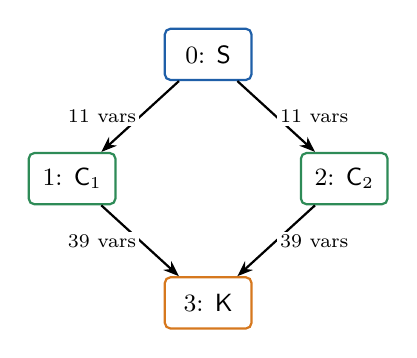
\begin{tikzpicture}[node distance=9mm and 6mm]
\node[dnode,draw=colS,thick] (s) {0: $\nS$};
\node[dnode,draw=colC,thick,below left=of s] (c1) {1: $\nC_1$};
\node[dnode,draw=colC,thick,below right=of s] (c2) {2: $\nC_2$};
\node[dnode,draw=colK,thick,below right=of c1] (k) {3: $\nK$};
\draw[sedge] (s) -- node[elab,left] {11 vars} (c1);
\draw[sedge] (s) -- node[elab,right] {11 vars} (c2);
\draw[sedge] (c1) -- node[elab,left] {39 vars} (k);
\draw[sedge] (c2) -- node[elab,right] {39 vars} (k);
\end{tikzpicture}
\end{minipage}
\caption{A complete Dagster DAG file (long lines shortened) and the graph it describes. This
is the top-down decomposition of depth 1 (\cref{sec:topdown}) of the smallest benchmark
instance ($N=8$: 221 variables, 1{,}111 clauses). Node~0 sends each of nodes~1 and~2 an
11-bit sub-target. Each of them returns 11 summary bits plus 28 transcript-choice variables
to node~3. Nodes~0 and~3 hold the same clauses.}
\label{fig:dagfile}
\end{figure}

\subsection{Execution: one master, many workers}
\label{sec:execution}
Dagster runs as $R$ MPI processes (\emph{ranks}). Rank~0 is the \emph{master}; ranks
$1,\dots,R-1$ are the $P=R-1$ \emph{workers}. \Cref{fig:arch} shows the cycle:
\begin{enumerate}
\item \textbf{Combination.} For every edge $e$ the master keeps a \emph{message table},
      the set of distinct messages produced so far on $e$. For a node $v$ with several
      incoming edges, it searches the Cartesian product of its incoming tables for
      combinations not yet dispatched. In the default table master (option \opt{-g 0})
      the search also checks that the chosen messages agree on any variable they share,
      comparing them literal by literal. Other values of \opt{-g} select a binary
      decision diagram (BDD) master (\opt{-g 1}) or the same table master \emph{without}
      the consistency check (any other value, e.g.\ \opt{-g 2}).
\item \textbf{Allocation.} New combinations become pending jobs in a buffer of at most $P$
      entries, and idle workers are assigned pending jobs. With option \opt{-b 0}, the
      master prefers jobs at nodes deeper in the DAG (depth-first). When there are
      \emph{more idle workers than pending jobs}, idle workers receive \emph{copies}
      (duplicates) of jobs already being worked on. This guards against a slow worker,
      but, as \cref{sec:dup} shows, it can be expensive.
\item \textbf{Solving.} A worker builds the clause set $F_v$ of its node and adds the input
      $\alpha_{\text{in}}$ as unit clauses. It then runs a SAT engine (option \opt{-m};
      \opt{-m 4} selects MiniSat) and sends the solution back.
\item \textbf{Recording.} For each outgoing edge, the master restricts the solution to that
      edge's interface variables and adds the result to the edge's message table if it is
      new.
\item \textbf{Termination.} The enumeration mode \opt{-e} controls how many solutions are
      sought. With \opt{-e 3}, used throughout this study, a worker returns \emph{one}
      solution per job and then asks for new work, and the master stops at the first
      terminal solution. It writes that solution to the file given by \opt{-o}.
\end{enumerate}

\begin{figure}[htbp]
\centering
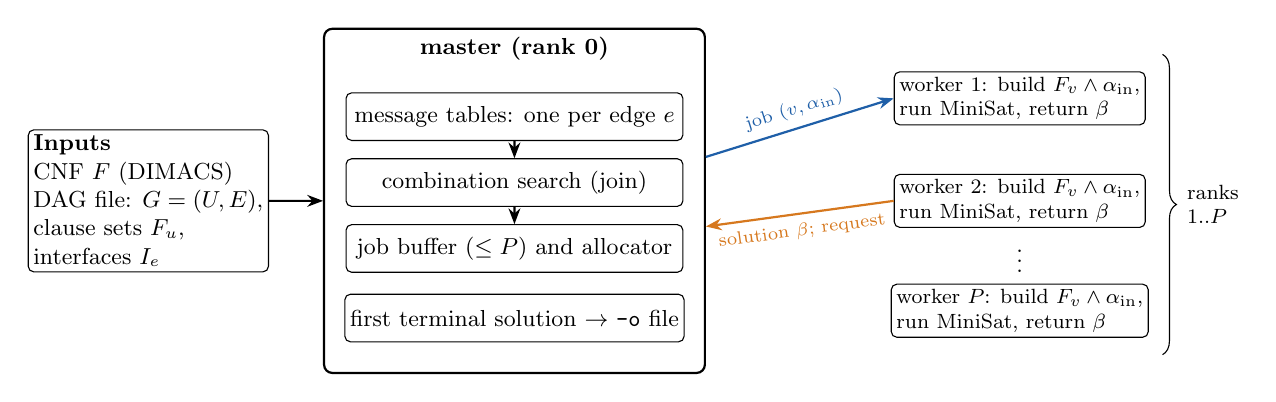
\begin{tikzpicture}[font=\small, scale=0.93, transform shape]
\node[dnode, minimum width=24mm, align=left] (in) at (-0.3,0)
  {\textbf{Inputs}\\ CNF $F$ (DIMACS)\\ DAG file: $G=(U,E)$,\\ clause sets $F_u$,\\ interfaces $I_e$};
\node[draw, rounded corners=3pt, thick, minimum width=52mm, minimum height=47mm] (m) at (4.7,0) {};
\node[anchor=north, font=\small\bfseries] at (m.north) {master (rank 0)};
\node[dnode, minimum width=46mm] (t) at (4.7,1.15) {message tables: one per edge $e$};
\node[dnode, minimum width=46mm] (c) at (4.7,0.25) {combination search (join)};
\node[dnode, minimum width=46mm] (b) at (4.7,-0.65) {job buffer ($\le P$) and allocator};
\node[dnode, minimum width=46mm, align=center] (o) at (4.7,-1.6) {first terminal solution $\to$ \opt{-o} file};
\draw[sedge] (t) -- (c); \draw[sedge] (c) -- (b);
\foreach \k/\y in {1/1.4, 2/0.0, P/-1.5} {
  \node[dnode, align=left, font=\footnotesize] (w\k) at (11.6,\y)
    {worker $\k$: build $F_v\land\alpha_{\mathrm{in}}$,\\ run MiniSat, return $\beta$};
}
\node at (11.6,-0.72) {$\vdots$};
\draw[decorate,decoration={brace,amplitude=5pt}] (13.55,2.0) -- (13.55,-2.1)
  node[midway, right=6pt, align=left, font=\footnotesize] {ranks\\$1..P$};
\draw[sedge] (in) -- (m.west);
\draw[sedge, colS] ($(m.east)+(0,0.6)$) -- node[font=\scriptsize, above, sloped, text=colS] {job $(v,\alpha_{\mathrm{in}})$} (w1.west);
\draw[sedge, colK] (w2.west) -- node[font=\scriptsize, below, sloped, text=colK] {solution $\beta$; request} ($(m.east)+(0,-0.35)$);
\end{tikzpicture}
\caption{Dagster's execution model. The master keeps one table of distinct messages per edge,
searches for unseen combinations of incoming messages, and hands the resulting jobs to idle
workers. Each worker solves its node's clauses under the given input and returns a solution;
the master records the solution's restriction to every outgoing edge as new messages. All
traffic goes through the master.}
\label{fig:arch}
\end{figure}

\paragraph{What a terminal solution guarantees.}
A terminal solution is consistent with its input messages. Each of those messages came from
a solution consistent with \emph{its} inputs, and so on back to the sources. Whether this
chain amounts to a model of the whole formula $F$ depends on the DAG: every clause must be
held by some node, and every variable shared between nodes' clause sets must travel along
the edges. \Cref{sec:families} argues this for each decomposition. Independently of that
argument, every answer in our experiments was \emph{checked}: we rebuilt a full assignment
from the reported transcript choices and evaluated every clause of $F$ and the attack
condition (\cref{sec:verification}).

\paragraph{Logging.}
Dagster logs through the glog library at a configurable verbosity. At verbosity~2 the
master logs every job it dispatches and every request for work it receives. At
verbosity~3 it also logs every solution it receives and its internal statistics, and
workers log when they finish a job. All timestamps have microsecond resolution. Our
analysis of where time goes (\cref{sec:results}) is reconstructed entirely from these logs.

\begin{table}[htbp]
\centering\small
\begin{tabular}{@{}lp{0.68\textwidth}@{}}
\toprule
Option & Meaning, and the value used in this study \\
\midrule
\opt{-m 4}  & SAT engine for every node: MiniSat (other values select TiniSAT and local-search helpers) \\
\opt{-e 3}  & one solution per job; stop at the first terminal solution \\
\opt{-b 0}  & depth-first scheduling: prefer jobs at nodes deeper in the DAG \\
\opt{-g 0} / \opt{-g 2} & table master with / without the literal-by-literal consistency check of combinations (\cref{sec:joincheck}); \opt{-g 2} from \cref{sec:joincheck} on \\
\opt{-o} \textit{file} & where the terminal solution is written \\
\texttt{mpirun -n} $R$ & number of ranks: one master and $P=R-1$ workers, one rank per core \\
\bottomrule
\end{tabular}
\caption{Dagster options used in this study.}
\label{tab:options}
\end{table}

% ======================================================================
\section{The benchmark: an XOR session attack (\XSA)}
\label{sec:xsa}

\subsection{The attack scenario}
Consider a protocol in which each \emph{session} (or \emph{episode}) between honest parties
produces a transcript. A fixed function turns the transcript into a $W$-bit word that
contributes to a checksum by exclusive-or. XOR-based checksums and MACs are a classic source
of such linear structure. An adversary who has observed or can induce several transcripts
per session may choose \emph{which} transcript of each session to use. The question is
whether the adversary can choose one transcript per session so that the XOR of all
contributions equals a \emph{target fingerprint}, for instance the checksum of a message
they wish to forge. \XSA{} is a synthetic benchmark that captures exactly this combinatorial
core, with a single scale parameter $N$.
It is \emph{not} a symbolic protocol model: sessions and transcripts only interpret
the list structure. Roles, network deduction, keys and concrete cryptography are not modelled.

\subsection{The problem, formally}
\label{sec:xsa-formal}
Let $N$ be the number of episodes, indexed $i=0,\dots,N-1$. Each episode offers
$Q$ transcripts, indexed $j=0,\dots,Q-1$. Choosing transcript $j$ in episode $i$
contributes the \emph{delta} $\delta_{i,j}\in\{0,1\}^W$, a $W$-bit word. Given a target
$t\in\{0,1\}^W$, the problem asks for a \emph{selection} $s=(s_0,\dots,s_{N-1})$ with
$s_i\in\{0,\dots,Q-1\}$ such that
\begin{equation}
\delta_{0,s_0}\oplus\delta_{1,s_1}\oplus\dots\oplus\delta_{N-1,s_{N-1}} \;=\; t,
\label{eq:attack}
\end{equation}
where $\oplus$ is bitwise XOR. The generator derives every other parameter from $N$:
\begin{equation}
Q(N) = 4 + \lceil\log_2 N\rceil, \qquad W(N) = 8 + \lceil\log_2 N\rceil.
\label{eq:qw}
\end{equation}
The deltas are distinct non-zero words obtained from SHA-256 of a fixed tag, so every
instance is reproducible. The generator also draws a \emph{planted} selection and sets $t$
to its XOR, which guarantees at least one solution.

\paragraph{How many solutions? A random-XOR predictor.}
There are $Q^N$ selections and $2^W$ possible XOR values. If the deltas behaved like
independent uniformly random words, a fixed target would be hit by about
\begin{equation}
\widehat{\lambda}(k) = Q^{k}/2^{W}
\label{eq:lambda}
\end{equation}
selections of any $k$ episodes. The hat marks a model quantity: the real deltas are
deterministic (truncated SHA-256 values, with zero and duplicate words repaired), and the
target is planted. For the whole instance $\widehat{\lambda}(N)$ is astronomically large, so
solutions are plentiful, and the difficulty for a SAT solver lies entirely in finding one
through the XOR structure. Equation~\eqref{eq:attack} is an instance of the multi-list XOR
problem studied by Wagner~\cite{wagner2002birthday}, with $N$ lists of size $Q$. The
\emph{birthday regime}, in which solutions are scarce, is discussed in \cref{sec:xsab}.

\subsection{The semantic tree and its CNF encoding}
\label{sec:encoding}
The generator organises the XOR in~\eqref{eq:attack} as a balanced binary tree, the
\emph{semantic tree} (\cref{fig:xsa}):
\begin{itemize}
\item Its leaves are the \emph{episode nodes} $\varepsilon_0,\dots,\varepsilon_{N-1}$.
\item Each internal \emph{join node} XORs the $W$-bit \emph{summaries} of its two children.
      Joins are named \texttt{join\_L$h$\_$i_0$\_$i_1$}: a join at level $h$ covers the
      $2^{h+1}$ episodes $i_0,\dots,i_1-1$.
\item A \emph{goal node} $\gamma$ requires the root's summary to equal $t$.
\end{itemize}
For a semantic node $n$, we write $\outb(n)$ for its $W$ summary bits, $\lv(n)$ for the set
of episodes below it, and $\selv(n)$ for the selector variables of those episodes.
\Cref{tab:gadgets} lists the variables and clauses of each kind of node.
The episode clauses are one-directional implications, ``if transcript $j$ is chosen then the
summary equals $\delta_{i,j}$'', yet they encode the episode exactly. Exactly one selector
$x_{i,j}$ is true, so the implications of that one transcript fix every summary bit, and the
implications of unselected transcripts are vacuous. No reverse implication is needed.

\begin{figure}[htbp]
\centering
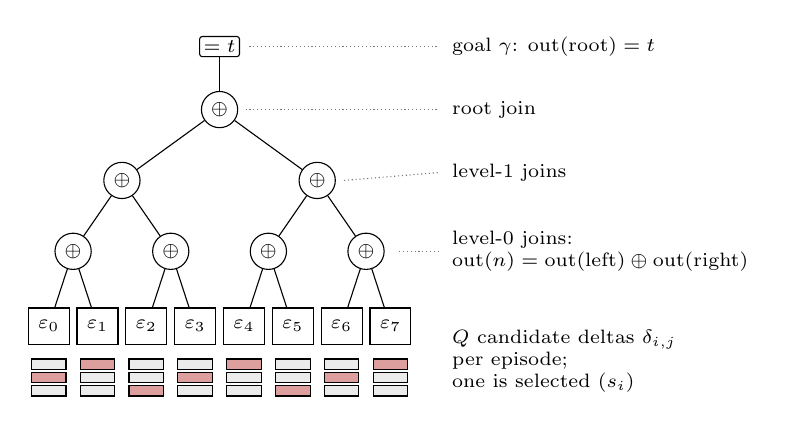
\begin{tikzpicture}
\pic (T) at (0,0) {semtree};
% delta stacks under the leaves
\foreach \i in {0,...,7} {
  \foreach \j in {0,1,2} { \draw[fill=colA!15] ($(T-l\i.south)+(-0.22,-0.18-0.17*\j)$) rectangle ++(0.44,-0.13); }
  \pgfmathtruncatemacro{\chosen}{mod(2*\i+1,3)}
  \draw[fill=colR!55] ($(T-l\i.south)+(-0.22,-0.18-0.17*\chosen)$) rectangle ++(0.44,-0.13);
}
\node[font=\scriptsize, align=left, anchor=west] at (5.0,-0.45) {$Q$ candidate deltas $\delta_{i,j}$\\ per episode;\\ one is selected ($s_i$)};
\node[font=\scriptsize, align=left, anchor=west] at (5.0,0.95) {level-0 joins:\\ $\outb(n)=\outb(\text{left})\oplus\outb(\text{right})$};
\node[font=\scriptsize, align=left, anchor=west] at (5.0,1.95) {level-1 joins};
\node[font=\scriptsize, align=left, anchor=west] at (5.0,2.75) {root join};
\node[font=\scriptsize, align=left, anchor=west] at (5.0,3.55) {goal $\gamma$: $\outb(\text{root}) = t$};
\draw[densely dotted, colA] (4.45,0.95) -- (4.95,0.95);
\draw[densely dotted, colA] (3.75,1.85) -- (4.95,1.95);
\draw[densely dotted, colA] (2.5,2.75) -- (4.95,2.75);
\draw[densely dotted, colA] (2.55,3.55) -- (4.95,3.55);
\end{tikzpicture}
\caption{The \XSA{} problem for $N=8$, drawn as its semantic tree. Each episode $\varepsilon_i$
selects one of $Q$ candidate $W$-bit deltas (red: the selected one). Each join ($\oplus$)
XORs the $W$-bit summaries of its children. The goal requires the root's summary to equal
the target $t$. The real instances in this study have $N=2048$ to $16384$ episodes, i.e.\
11 to 14 join levels.}
\label{fig:xsa}
\end{figure}

\begin{table}[htbp]
\centering\small
\begin{tabular}{@{}p{0.16\textwidth}p{0.39\textwidth}p{0.38\textwidth}@{}}
\toprule
Node & Variables and meaning & Clauses \\
\midrule
episode $\varepsilon_i$ & selectors $x_{i,0},\dots,x_{i,Q-1}$ ($x_{i,j}$: ``transcript $j$ is used'');
  summary bits $y_{\varepsilon_i,0},\dots,y_{\varepsilon_i,W-1}$ &
  exactly one $x_{i,j}$: $1+\binom{Q}{2}$; for every $j$ and bit $b$: $(\neg x_{i,j}\lor y_{\varepsilon_i,b})$ if bit $b$ of $\delta_{i,j}$ is 1, else $(\neg x_{i,j}\lor\neg y_{\varepsilon_i,b})$: $QW$ \\
join $n$ with children $n_1,n_2$ & summary bits $y_{n,b}$, $b<W$ &
  $W$ XOR gates $y_{n,b}\leftrightarrow y_{n_1,b}\oplus y_{n_2,b}$: $4W$ \\
goal $\gamma$ & none (constrains the root's bits) & $W$ unit clauses fixing $\outb(\text{root})=t$ \\
\bottomrule
\end{tabular}
\caption{The CNF gadgets of \XSA{}, built from the exactly-one and XOR encodings of
\cref{sec:encodings}.}
\label{tab:gadgets}
\end{table}

\paragraph{Size.}
Summing the gadgets over the $N$ episodes, $N-1$ joins and the goal gives
\begin{align}
|V| &= N\,(Q+2W) - W,\label{eq:nvars}\\
|F| &= N\left(1+\tbinom{Q}{2}+QW\right) + 4W(N-1) + W.\label{eq:nclauses}
\end{align}
These formulas reproduce the headers of the generated files exactly (\cref{tab:instances}).
The DIMACS file is \emph{shuffled}: variable numbers and clause order are permuted, so the
solver cannot see the tree. A separate metadata file records which clauses and variables
belong to which semantic node. Our decompositions use that metadata.

\begin{table}[htbp]
\centering\small
\begin{tabular}{@{}rrrrrl@{}}
\toprule
$N$ & $Q$ & $W$ & variables $|V|$ & clauses $|F|$ & single-solver baseline (one-node Dagster, cluster) \\
\midrule
2{,}048 & 15 & 19 & 108{,}525 & 956{,}359 & 174.3\,s \\
4{,}096 & 16 & 20 & 229{,}356 & 2{,}133{,}956 & did not finish in 3{,}600\,s \\
8{,}192 & 17 & 21 & 483{,}307 & 4{,}734{,}913 & not run (would exceed many hours) \\
16{,}384 & 18 & 22 & 1{,}015{,}786 & 10{,}452{,}926 & not run \\
\bottomrule
\end{tabular}
\caption{The \XSA{} instances used on the cluster, with sizes from \cref{eq:nvars,eq:nclauses}.}
\label{tab:instances}
\end{table}

\paragraph{Why it is hard for one solver.}
On a single core, MiniSat inside one-node Dagster took 174\,s for $N=2048$ and did not
finish within an hour for $N=4096$. Plain MiniSat run on the $N=2048$ file with different
random seeds took between 35\,s and 156\,s, which illustrates the heavy tail. The growth
with $N$ is steep, although the instance stays linear in size.

\subsection{A worked example: $N=2$}
\label{sec:example}
Take $N=2$ episodes, $Q=2$ transcripts and $W=3$ bits, with the deltas below (words written
with bit~2 first). Of the eight possible targets, exactly four are reachable: the four
selections give four distinct XORs. That is $\widehat{\lambda}(2)=2^2/2^3=\tfrac12$ in
miniature. We choose the reachable target $t=100$.
\begin{center}\small
\begin{tabular}{@{}lcc@{}}
\toprule
deltas & $j=0$ & $j=1$\\
\midrule
episode 0 & $\delta_{0,0}=001$ & $\delta_{0,1}=110$\\
episode 1 & $\delta_{1,0}=010$ & $\delta_{1,1}=111$\\
\bottomrule
\end{tabular}
\qquad
\begin{tabular}{@{}cc@{}}
\toprule
selection $(s_0,s_1)$ & $\delta_{0,s_0}\oplus\delta_{1,s_1}$\\
\midrule
$(0,0)$ & $011$\\ $(0,1)$ & $110$\\ $(1,0)$ & $\mathbf{100}$\\ $(1,1)$ & $001$\\
\bottomrule
\end{tabular}
\end{center}
By \cref{eq:nvars,eq:nclauses} the CNF has $2(2+6)-3=13$ variables and
$2(1+1+6)+12+3=31$ clauses. Number the variables
$x_{0,0},x_{0,1},x_{1,0},x_{1,1}$ as 1--4; the summary bits $y_{\varepsilon_0,b}$ as 5--7 and
$y_{\varepsilon_1,b}$ as 8--10 ($b=0,1,2$); and the root's bits as 11--13. The clauses are:
\begin{itemize}
\item \textbf{Exactly one transcript per episode} (4 clauses): $(x_{0,0}\lor x_{0,1})$,
      $(\neg x_{0,0}\lor\neg x_{0,1})$, and the same for episode~1.
\item \textbf{Leaf implications} (12 clauses). For $\delta_{0,0}=001$:
      $(\neg x_{0,0}\lor y_{\varepsilon_0,0})$, $(\neg x_{0,0}\lor\neg y_{\varepsilon_0,1})$,
      $(\neg x_{0,0}\lor\neg y_{\varepsilon_0,2})$. Likewise for the other three deltas.
\item \textbf{One join} (12 clauses): three XOR gates
      $y_{r,b}\leftrightarrow y_{\varepsilon_0,b}\oplus y_{\varepsilon_1,b}$.
\item \textbf{Goal} (3 clauses): $(\neg y_{r,0})$, $(\neg y_{r,1})$, $(y_{r,2})$, i.e.\
      the root equals $100$.
\end{itemize}
The unique model sets $x_{0,1}=x_{1,0}=1$ and the other selectors to 0. Propagation then gives
$\outb(\varepsilon_0)=110$, $\outb(\varepsilon_1)=010$ and $\outb(\text{root})=100$, and every
clause is satisfied. \Cref{sec:topdown} returns to this example to show what a top-down
decomposition sends along its edges.

\subsection{The birthday regime (\XSAB)}
\label{sec:xsab}
A companion prototype, \XSAB, keeps the same CNF shape but chooses parameters so that
solutions are \emph{scarce}. It uses $N=2^m$ episodes, $Q=2^\omega$ choices (with
$\omega=4$) and $W=\omega(m+1)$ bits, which is Wagner's balance for the multi-list
problem~\cite{wagner2002birthday}. Wagner's tree algorithm solves such instances by
\emph{filtration}: a join at level $h$ keeps only those partial XORs whose next block of
$\omega$ bits is zero (\cref{fig:xsab}). The prototype therefore writes two CNFs with
identical numbering:
\begin{itemize}
\item a \emph{plain} CNF, which is the problem itself;
\item a \emph{strategy} CNF, which adds Wagner's filtration as unit clauses on each join's
      next $\omega$ summary bits.
\end{itemize}
The strategy is a heuristic that restricts which solutions are sought; it is not part of
the problem.

\begin{figure}[htbp]
\centering
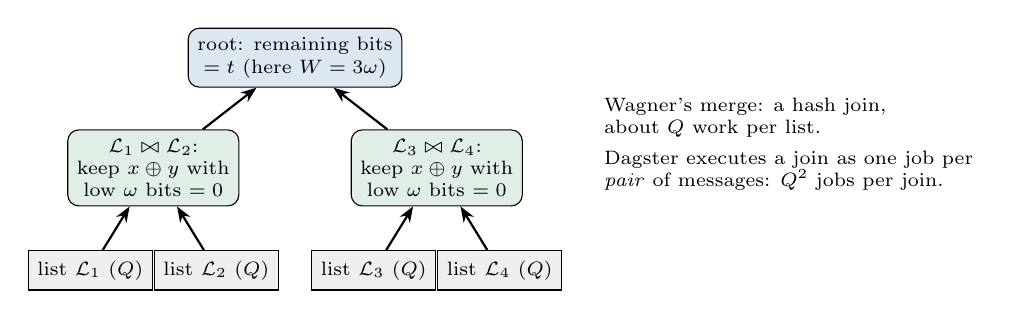
\begin{tikzpicture}[font=\scriptsize]
\foreach \i/\x in {1/0,2/1.6,3/3.6,4/5.2} {
  \node[draw, minimum width=12mm, minimum height=5mm, fill=colA!12] (L\i) at (\x,0) {list $\mathcal{L}_\i$ ($Q$)};
}
\node[draw, rounded corners, fill=colC!15, align=center] (J1) at (0.8,1.3) {$\mathcal{L}_1\bowtie\mathcal{L}_2$:\\ keep $x\oplus y$ with\\ low $\omega$ bits $=0$};
\node[draw, rounded corners, fill=colC!15, align=center] (J2) at (4.4,1.3) {$\mathcal{L}_3\bowtie\mathcal{L}_4$:\\ keep $x\oplus y$ with\\ low $\omega$ bits $=0$};
\node[draw, rounded corners, fill=colS!15, align=center] (R) at (2.6,2.7) {root: remaining bits\\ $= t$ (here $W=3\omega$)};
\draw[sedge] (L1) -- (J1); \draw[sedge] (L2) -- (J1); \draw[sedge] (L3) -- (J2); \draw[sedge] (L4) -- (J2);
\draw[sedge] (J1) -- (R); \draw[sedge] (J2) -- (R);
\node[align=left, anchor=west] at (6.4,1.6) {Wagner's merge: a hash join,\\ about $Q$ work per list.\\[3pt]
  Dagster executes a join as one job per\\ \emph{pair} of messages: $Q^2$ jobs per join.};
\end{tikzpicture}
\caption{Wagner's tree algorithm for four lists (\XSAB{} with $m=2$), shown with zero
targets at the inner joins; the generator also handles a non-zero target along the tree's
right spine. Filtration at each join keeps only partial XORs that vanish on the next $\omega$
bits. The \XSAB{} ``strategy'' CNF adds these filtration conditions as unit clauses.}
\label{fig:xsab}
\end{figure}

\paragraph{What \XSAB{} showed.}
The measurements below are from one core in a development sandbox:
\begin{itemize}
\item \textbf{Plain CNF:} flat MiniSat grows about 10$\times$ per doubling of $N$, from
      0.45\,s at $N=16$ to over 90\,s at $N=64$.
\item \textbf{Strategy CNF:} the \emph{same flat solver} solves every size tried, for
      example $N=128$ in 1.7\,s.
\item \textbf{Wagner's tree as a Dagster DAG}, run over the strategy CNF, is about
      $100\times$ slower than the flat solver with the same clauses. It ran 4{,}083 jobs at
      $N=16$ and 8{,}083 at $N=32$, which matches one job per \emph{pair} of messages:
      $(N-1)Q^2$ plus the leaves.
\item \textbf{Fusing the lower levels into blocks} (\cref{sec:early}) cut this to 25 jobs at
      $N=16$.
\end{itemize}
The lesson, which recurs throughout this report, is that knowledge a decomposition encodes
(a filtration, a pinned prefix) usually helps a flat solver just as much once written as
clauses. A decomposition must therefore be compared with \emph{the flat solver given the
same knowledge}.

% ======================================================================
\section{Decomposing \XSA{} for Dagster}
\label{sec:families}

A \emph{decomposition} maps the semantic tree onto a Dagster DAG. It decides which semantic
nodes' clauses each Dagster node holds, and which variables travel along each edge. We call
a parameterised way of doing this a DAG \emph{family} and name it as in our tools, e.g.\
\dfam{topdown:7}. Three questions decide whether a family is useful:
\begin{itemize}
\item \textbf{Does each join filter?} A node with several inputs runs one job per
      consistent combination of input messages. If the inputs share no variables, every
      combination is consistent, and the node turns into a nested loop.
\item \textbf{Does each piece succeed?} If a node can reject its input, the producer must be
      able to offer alternatives.
\item \textbf{Does it beat the flat solver given the same knowledge?} If not, the gain is an
      algorithmic shortcut rather than distribution.
\end{itemize}

\subsection{Early families: one node, split, semantic tree, blocks}
\label{sec:early}
\Cref{fig:early} shows the four families explored first. They were evaluated on one core
in a development sandbox, with Dagster enumerating solutions (its default mode).

\begin{itemize}
\item \textbf{\dfam{one}.} A single node holds all of $F$, so Dagster reduces to one
      MiniSat run. This is the baseline.

\item \textbf{\dfam{split:$K$}.} Follow the tree's right spine from the root down to the
      first subtree with at most $K$ episodes: the \emph{residual block}.
      \begin{itemize}
      \item Node~$\nB$ holds the residual block, the joins on its path to the root, and the
            goal.
      \item Node~$\nA$ holds everything else: the \emph{sibling} subtrees hanging off that
            path.
      \item The single edge $\nA\to\nB$ carries the siblings' summaries and selectors.
      \end{itemize}
      $\nA$ can complete any selection of its episodes trivially. $\nB$ must then find $K$
      choices that bring the XOR to $t$, which succeeds with probability
      $1-e^{-\widehat{\lambda}(K)}$ (about 100\% at $K=8$). At $N=2048$ this cut the sandbox time from
      185\,s to 6.9\,s. However, a \emph{cube control} showed why: pinning the same episodes
      to an arbitrary prefix with unit clauses lets flat MiniSat finish in 4.1\,s ($N=2048$)
      and 3.5\,s ($N=4096$, where \dfam{split:8} took 32\,s). The split's gain is a cube,
      not distribution.

\item \textbf{\dfam{tree}.} Every semantic node is a Dagster node. Each edge runs from child
      to parent and carries the child's summary bits and all selectors below it, so the
      goal can report the whole selection. Sibling subtrees share no variables, so a join
      sees every pair of child messages as consistent and dispatches each pair as a job. At
      $N=32$ the run made 9{,}206 jobs (8{,}965 at a single level-1 join) and timed out
      after 100\,s. One-node Dagster solved the same instance in 0.61\,s.

\item \textbf{\dfam{block:$B$}.} Subtrees with at most $B$ episodes are fused into one node
      each; the joins above them and the goal stay separate. At $N=8$, \dfam{block:4} needed
      11{,}519 jobs (74.9\,s). At $N=32$, \dfam{block:8} ran only 2 jobs in 100\,s: each
      block enumerated an endless stream of distinct selections and held its worker,
      starving the other blocks.
\end{itemize}

\begin{figure}[htbp]
\centering
\begin{subfigure}[b]{0.48\textwidth}\centering
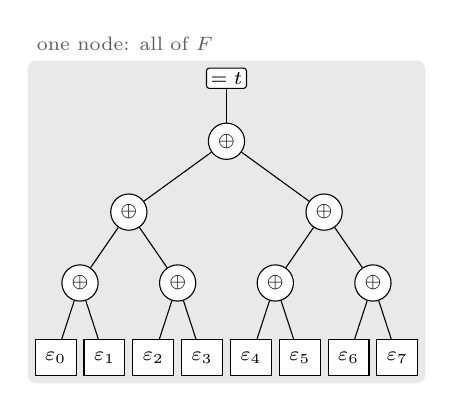
\begin{tikzpicture}
\pic (A) at (0,0) {semtree};
\begin{scope}[on background layer]
\node[region, fill=colA!18, fit=(A-l0)(A-l7)(A-g)] (ra) {};
\end{scope}
\node[font=\scriptsize, anchor=south west, text=colA!80!black] at (ra.north west) {one node: all of $F$};
\end{tikzpicture}
\caption{\dfam{one}}
\end{subfigure}\hfill
\begin{subfigure}[b]{0.48\textwidth}\centering
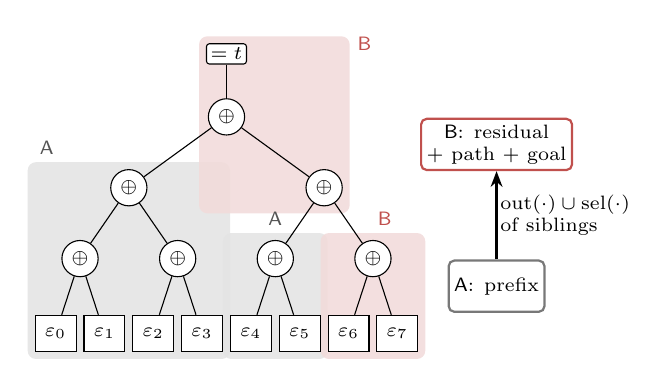
\begin{tikzpicture}
\pic (B) at (0,0) {semtree};
\begin{scope}[on background layer]
\node[region, fill=colA!20, fit=(B-l0)(B-l3)(B-a)] (a1) {};
\node[region, fill=colA!20, fit=(B-l4)(B-l5)(B-e)] (a2) {};
\node[region, fill=colR!20, fit=(B-l6)(B-l7)(B-f)] (b1) {};
\node[region, fill=colR!20, fit=(B-b)(B-r)(B-g)] (b2) {};
\end{scope}
\node[font=\scriptsize\bfseries, text=colA!70!black] at ($(a1.north west)+(0.25,0.18)$) {$\nA$};
\node[font=\scriptsize\bfseries, text=colA!70!black] at ($(a2.north)+(0,0.18)$) {$\nA$};
\node[font=\scriptsize\bfseries, text=colR] at ($(b1.north)+(0.15,0.18)$) {$\nB$};
\node[font=\scriptsize\bfseries, text=colR] at ($(b2.north east)+(0.18,-0.1)$) {$\nB$};
\node[dnode, draw=colA, thick, font=\scriptsize] (na) at (5.6,0.6) {$\nA$: prefix};
\node[dnode, draw=colR, thick, font=\scriptsize, align=center] (nb) at (5.6,2.4) {$\nB$: residual\\ + path + goal};
\draw[sedge] (na) -- node[elab, right, align=left] {$\outb(\cdot)\cup\selv(\cdot)$\\ of siblings} (nb);
\end{tikzpicture}
\caption{\dfam{split:$K$} (here $K=2$)}
\end{subfigure}

\vspace{4mm}
\begin{subfigure}[b]{0.48\textwidth}\centering
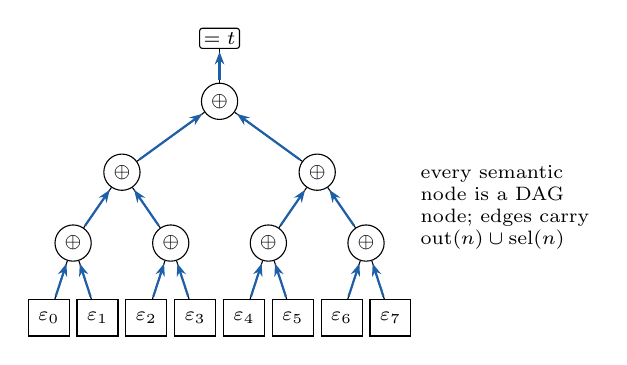
\begin{tikzpicture}
\pic (C) at (0,0) {semtree};
\foreach \p/\x in {c/l0,c/l1,d/l2,d/l3,e/l4,e/l5,f/l6,f/l7,a/c,a/d,b/e,b/f,r/a,r/b,g/r}
  { \draw[-{Stealth[length=1.6mm]}, colS, thick, shorten <=1pt, shorten >=1pt] (C-\x) -- (C-\p); }
\node[font=\scriptsize, align=left, anchor=west] at (4.6,1.4) {every semantic\\ node is a DAG\\ node; edges carry\\ $\outb(n)\cup\selv(n)$};
\end{tikzpicture}
\caption{\dfam{tree} (the semantic tree itself)}
\end{subfigure}\hfill
\begin{subfigure}[b]{0.48\textwidth}\centering
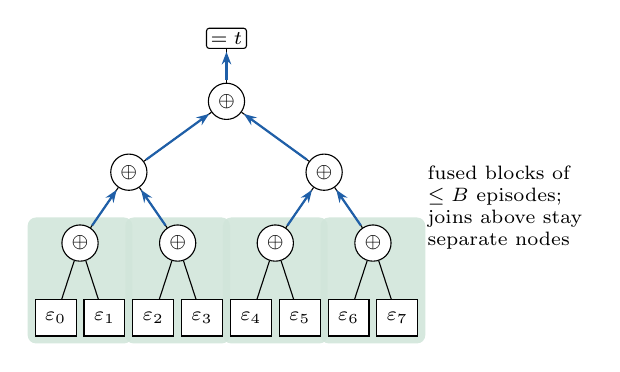
\begin{tikzpicture}
\pic (D) at (0,0) {semtree};
\begin{scope}[on background layer]
\foreach \s/\x/\y in {c/l0/l1, d/l2/l3, e/l4/l5, f/l6/l7}
  { \node[region, fill=colC!22, fit=(D-\x)(D-\y)(D-\s)] {}; }
\end{scope}
\foreach \p/\x in {a/c,a/d,b/e,b/f,r/a,r/b,g/r}
  { \draw[-{Stealth[length=1.6mm]}, colS, thick, shorten <=1pt, shorten >=1pt] (D-\x) -- (D-\p); }
\node[font=\scriptsize, align=left, anchor=west] at (4.6,1.4) {fused blocks of\\ $\le B$ episodes;\\ joins above stay\\ separate nodes};
\end{tikzpicture}
\caption{\dfam{block:$B$} (here $B=2$)}
\end{subfigure}
\caption{The four early families on an $N=8$ semantic tree. Shaded regions show which
semantic nodes' clauses each Dagster node holds; arrows are Dagster edges. In (b), the
residual block is the rightmost $K$-episode subtree, and node $\nB$ also holds the joins on
its path to the root and the goal. Results are summarised in \cref{tab:families}.}
\label{fig:early}
\end{figure}

\subsection{Top-down target splitting (\dfam{topdown:$D$})}
\label{sec:topdown}
The family that works turns the tree upside down. Instead of combining bottom-up, it first
\emph{chooses sub-targets} top-down, solves the subtrees independently, and finally
assembles the result. Fix a depth $D$. The $2^D$ semantic nodes at depth $D$ below the root
are the \emph{subtree roots} $c_1,\dots,c_{2^D}$, each covering $k=N/2^D$ episodes. The
joins above depth $D$ form the \emph{top region} $\mathcal{T}_D$. The DAG
(\cref{fig:topdown}) has $2^D+2$ nodes:
\begin{itemize}
\item \textbf{Splitter $\nS$} (node 0) holds $\mathcal{T}_D$ and the goal $\gamma$. Its
      solution assigns every $\outb(c_i)$, which amounts to choosing \emph{sub-targets}
      $\tau_i$ whose XOR is $t$.
\item \textbf{Subtrees $\nC_i$} hold all clauses below $c_i$. Edge $\nS\to\nC_i$ carries
      $\outb(c_i)$ ($W$ variables), so $\nC_i$ must find a selection of its $k$ episodes
      whose XOR is $\tau_i$. This is an independent, smaller \XSA{} instance with a fixed
      target.
\item \textbf{Collector $\nK$} (the last node, a sink) holds $\mathcal{T}_D$ and $\gamma$
      again. Edge $\nC_i\to\nK$ carries $\outb(c_i)\cup\selv(c_i)$ ($W+kQ$ variables).
      $\nK$ re-solves the top region with every subtree's result fixed, and its solution
      contains every selector, i.e.\ the whole attack.
\end{itemize}

\paragraph{Soundness.}
Let $\beta_i$ be $\nC_i$'s solution and $\beta_{\nK}$ the collector's. The subtrees' variables are
pairwise disjoint, and $\nC_i$ shares only $\outb(c_i)$ with $\nK$, which $\nK$ receives from
$\nC_i$. Every clause of $F$ lies in some $\nC_i$ or in $\nK$. Hence
$\beta_{\nK}\cup\beta_1\cup\dots\cup\beta_{2^D}$ is a model of $F$. The splitter's own solution
only proposes sub-targets and is not part of the model.

\paragraph{The acceptance floor: a predictor, checked empirically.}
Subtree $\nC_i$ succeeds only if some selection of its $k$ episodes hits $\tau_i$. Under the
random-XOR model of \cref{eq:lambda}, the number of such selections is roughly
Poisson-distributed with mean $\widehat{\lambda}(k)$. This gives the \emph{acceptance
predictor}
\begin{equation}
\pacc(k) = 1-e^{-\widehat{\lambda}(k)}, \qquad \Pall(D) = \pacc\!\left(N/2^D\right)^{2^D},
\label{eq:pacc}
\end{equation}
for the probability that one subtree, respectively all subtrees, reach their sub-targets.
It is \emph{not} a completeness guarantee for the deterministic generated instances:
\begin{itemize}
\item the deltas are fixed words, not random ones;
\item the splitter chooses sub-targets deterministically;
\item subtree outcomes need not be independent.
\end{itemize}
We used it as a design rule. Under \opt{-e 3} the splitter offers a single split, so a
failing subtree would end the run without an attack, and the depth must stay above the
\emph{acceptance floor} where $\Pall\approx 1$. \Cref{fig:acceptance} shows that the
predicted floor is sharp:
\begin{itemize}
\item subtrees of at least 8 episodes are predicted safe for all four instances;
\item subtrees of 4 episodes almost never all succeed.
\end{itemize}
The deepest predicted-safe depth is $D=8,9,10,11$ for $N=2048,4096,8192,16384$. The
prediction was then checked against every executed configuration. All 171 top-down runs on the
cluster had $\Pall=1$ to double precision. All 169 that finished returned a verified attack,
which requires every subtree to succeed; the other two timed out for an unrelated reason
(\cref{sec:joincheck}). In the sandbox, \dfam{topdown:3} at $N=32$ (4-episode subtrees,
$\Pall=0.85\%$) timed out, as predicted.

\paragraph{The worked example, split top-down.}
For the $N=2$ instance of \cref{sec:example}, \dfam{topdown:1} has four nodes:
\begin{itemize}
\item $\nS$ holds the single join and the goal (15 clauses);
\item $\nC_0$ and $\nC_1$ hold one episode each (8 clauses each);
\item $\nK$ holds the join and the goal again.
\end{itemize}
Suppose $\nS$ returns the split $\tau_0=110$, $\tau_1=010$, which is valid because
$110\oplus010=100$. Then:
\begin{itemize}
\item the message on $\nS\to\nC_0$ is $y_{\varepsilon_0}=110$;
\item $\nC_0$ solves with $x_{0,1}=1$ and sends $\nK$ the five literals
      $y_{\varepsilon_0}=110$, $x_{0,0}=0$, $x_{0,1}=1$;
\item $\nC_1$ likewise sends $y_{\varepsilon_1}=010$, $x_{1,0}=1$, $x_{1,1}=0$;
\item $\nK$ re-solves the join with both summaries fixed, finds the root equal to $100$, and
      its solution contains all four selectors: the attack.
\end{itemize}
Had $\nS$ returned $\tau_0=001$, $\tau_1=101$ instead, $\nC_1$ would have been unsatisfiable,
because no delta of episode~1 equals $101$, and the run would have ended without an answer.
Of the eight splits of $100$, only one is accepted. This subtree size ($k=1$) lies far below
the floor, and the example also shows that the predictor is only approximate here: it gives
$\Pall=(1-e^{-1/4})^2\approx 4.9\%$, against the exact $1/8=12.5\%$.

\begin{figure}[htbp]
\centering
\begin{subfigure}[b]{0.44\textwidth}\centering
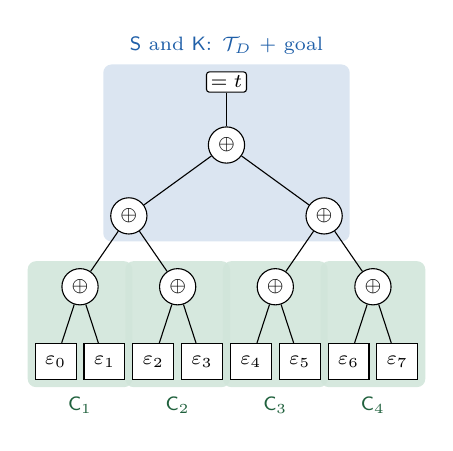
\begin{tikzpicture}
\pic (E) at (0,0) {semtree};
\begin{scope}[on background layer]
\node[region, fill=colS!18, fit=(E-a)(E-b)(E-r)(E-g)] (top) {};
\foreach \s/\x/\y/\n in {c/l0/l1/1, d/l2/l3/2, e/l4/l5/3, f/l6/l7/4}
  { \node[region, fill=colC!22, fit=(E-\x)(E-\y)(E-\s)] (s\n) {}; }
\end{scope}
\node[font=\scriptsize, text=colS, anchor=south] at (top.north) {$\nS$ and $\nK$: $\mathcal{T}_D$ + goal};
\foreach \n in {1,...,4} { \node[font=\scriptsize, text=colC!70!black] at ($(s\n.south)+(0,-0.22)$) {$\nC_{\n}$}; }
\end{tikzpicture}
\caption{regions for $N=8$, $D=2$}
\end{subfigure}\hfill
\begin{subfigure}[b]{0.54\textwidth}\centering
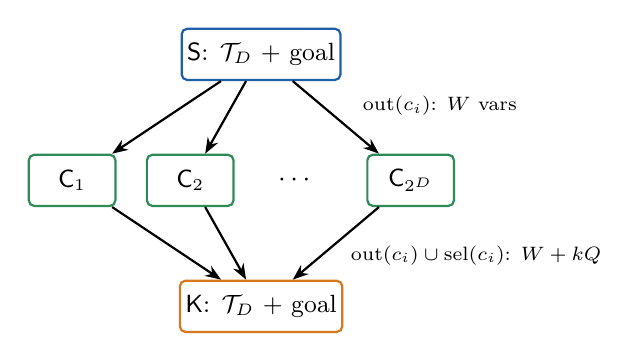
\begin{tikzpicture}[node distance=12mm]
\node[dnode, draw=colS, thick] (S) at (0,2.6) {$\nS$: $\mathcal{T}_D$ + goal};
\node[dnode, draw=colC, thick] (C1) at (-2.4,1.0) {$\nC_1$};
\node[dnode, draw=colC, thick] (C2) at (-0.9,1.0) {$\nC_2$};
\node at (0.45,1.0) {$\cdots$};
\node[dnode, draw=colC, thick] (Cn) at (1.9,1.0) {$\nC_{2^D}$};
\node[dnode, draw=colK, thick] (K) at (0,-0.6) {$\nK$: $\mathcal{T}_D$ + goal};
\foreach \c in {C1,C2,Cn} { \draw[sedge] (S) -- (\c); \draw[sedge] (\c) -- (K); }
\node[elab, anchor=west] at (1.25,1.95) {$\outb(c_i)$: $W$ vars};
\node[elab, anchor=west] at (1.1,0.05) {$\outb(c_i)\cup\selv(c_i)$: $W+kQ$};
\end{tikzpicture}
\caption{the DAG}
\end{subfigure}
\caption{Top-down target splitting, \dfam{topdown:$D$}. The splitter $\nS$ chooses a
sub-target for each of the $2^D$ subtrees. The subtrees $\nC_i$ are independent smaller
attacks with fixed targets. The collector $\nK$ re-checks the top region and gathers every
selector. $\nS$ and $\nK$ hold the same clauses.}
\label{fig:topdown}
\end{figure}

\begin{figure}[htbp]
\centering
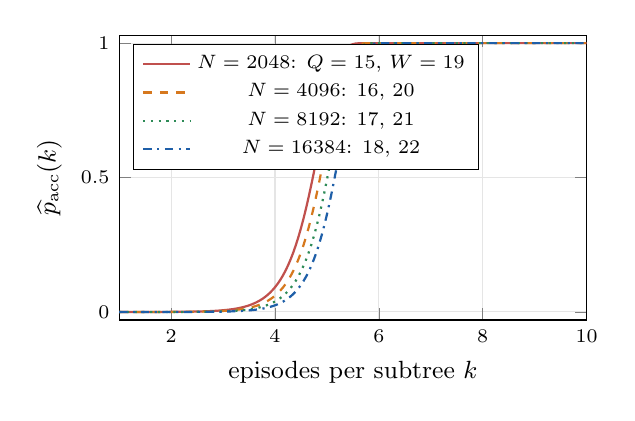
\begin{tikzpicture}
\begin{axis}[width=0.62\textwidth, height=5.2cm, xmin=1, xmax=10, ymin=-0.03, ymax=1.03,
  xlabel={episodes per subtree $k$}, ylabel={$\pacc(k)$}, legend pos=north west,
  legend style={font=\scriptsize}, tick label style={font=\scriptsize}, label style={font=\small},
  grid=major, grid style={gray!20}]
\addplot[colR, thick, domain=1:10, samples=181] {1-exp(-min((15^x)/2^19,50))};
\addplot[colK, thick, dashed, domain=1:10, samples=181] {1-exp(-min((16^x)/2^20,50))};
\addplot[colC, thick, dotted, domain=1:10, samples=181] {1-exp(-min((17^x)/2^21,50))};
\addplot[colS, thick, dashdotted, domain=1:10, samples=181] {1-exp(-min((18^x)/2^22,50))};
\legend{{$N=2048$: $Q=15$, $W=19$},{$N=4096$: $16$, $20$},{$N=8192$: $17$, $21$},{$N=16384$: $18$, $22$}}
\end{axis}
\end{tikzpicture}
\caption{The acceptance floor as predicted by \cref{eq:pacc}: the random-XOR estimate of the
probability that a $k$-episode subtree can reach a given $W$-bit sub-target. At $k=4$, $\pacc<10\%$, and with hundreds of
subtrees $\Pall\approx 0$. At $k=8$, $\pacc$ equals 1 to within $10^{-1000}$ for every
instance. All top-down runs on the cluster used $k\ge 8$.}
\label{fig:acceptance}
\end{figure}

\paragraph{Variants needing modified Dagster.}
Two variants were studied in the sandbox with small opt-in patches, and are not used on
the cluster (\cref{fig:variants}). Both target the case where the splitter \emph{streams} many
splits (enumeration rather than \opt{-e 3}):
\begin{itemize}
\item \textbf{Keyed edges} make every edge also carry the whole split
      $\kappa=(\outb(c_1),\dots,\outb(c_{2^D}))$, so that the collector only combines
      subtree results that belong to the same split.
\item \textbf{A bounded splitter} adds unit clauses that pin all but the lowest $\eta$ bits
      of the first $2^D-1$ sub-targets. The splitter can then offer at most
      $2^{\eta(2^D-1)}$ splits, so its stream ends.
\end{itemize}
They showed that a streaming splitter feeding siblings needs \emph{both} a join key and fair
scheduling of siblings. Under \opt{-e 3}, which needs neither, the plain family is simpler
and sufficient.

\begin{figure}[htbp]
\centering
\begin{subfigure}[b]{0.48\textwidth}\centering
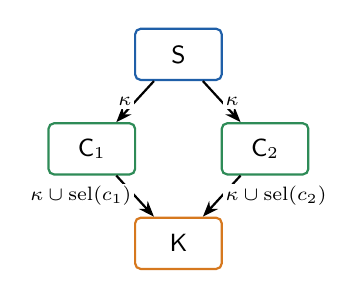
\begin{tikzpicture}
\node[dnode, draw=colS, thick] (S) at (0,2.2) {$\nS$};
\node[dnode, draw=colC, thick] (C1) at (-1.1,1.0) {$\nC_1$};
\node[dnode, draw=colC, thick] (C2) at (1.1,1.0) {$\nC_2$};
\node[dnode, draw=colK, thick] (K) at (0,-0.2) {$\nK$};
\draw[sedge] (S) -- node[elab, left] {$\kappa$} (C1); \draw[sedge] (S) -- node[elab, right] {$\kappa$} (C2);
\draw[sedge] (C1) -- node[elab, left] {$\kappa\cup\selv(c_1)$} (K); \draw[sedge] (C2) -- node[elab, right] {$\kappa\cup\selv(c_2)$} (K);
\end{tikzpicture}
\caption{keyed: every edge carries the whole split $\kappa$}
\end{subfigure}\hfill
\begin{subfigure}[b]{0.48\textwidth}\centering
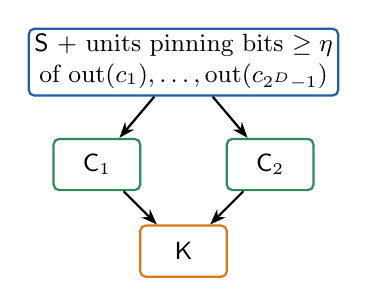
\begin{tikzpicture}
\node[dnode, draw=colS, thick, align=center] (S) at (0,2.2) {$\nS$ + units pinning bits $\ge\eta$\\ of $\outb(c_1),\dots,\outb(c_{2^D-1})$};
\node[dnode, draw=colC, thick] (C1) at (-1.1,0.9) {$\nC_1$};
\node[dnode, draw=colC, thick] (C2) at (1.1,0.9) {$\nC_2$};
\node[dnode, draw=colK, thick] (K) at (0,-0.2) {$\nK$};
\draw[sedge] (S) -- (C1); \draw[sedge] (S) -- (C2); \draw[sedge] (C1) -- (K); \draw[sedge] (C2) -- (K);
\end{tikzpicture}
\caption{bounded: at most $2^{\eta(2^D-1)}$ splits}
\end{subfigure}
\caption{Variants of top-down splitting for streaming splitters, studied with opt-in
Dagster patches (sandbox only; not used on the cluster).}
\label{fig:variants}
\end{figure}

\subsection{Two-stage top-down splitting (\dfam{topdown2:$d_1$:$d_2$})}
\label{sec:topdown2}
The final family stages the split, for a reason that only appeared at scale
(\cref{sec:dup}). With total depth $D=d_1+d_2$, the subtrees and the collector are exactly
those of \dfam{topdown:$D$}. Only the splitting changes (\cref{fig:topdown2}):
\begin{itemize}
\item \textbf{Top splitter $\nS$} holds the joins above depth $d_1$ and the goal. It chooses a
      sub-target for each of the $J=2^{d_1}$ \emph{block roots} $\hat c_1,\dots,\hat c_J$.
\item \textbf{Middle splitter $\nM_q$} holds the joins of block $q$ from depth $d_1$ down to
      depth $D$. Given $\outb(\hat c_q)$, it chooses sub-targets for the $2^{d_2}$ subtrees of
      its block. Any value of $\outb(\hat c_q)$ can be split, so $\nM_q$ always succeeds.
\item \textbf{Subtrees} $\nC_{q,1},\dots,\nC_{q,2^{d_2}}$ and the \textbf{collector} $\nK$ are
      as before. $\nK$ holds $\mathcal{T}_D$ and the goal.
\end{itemize}
There are $1+2^{d_1}+2^{D}+1$ nodes. The soundness argument and the acceptance floor are
unchanged. What changes is the size of each splitter's solution: $\nS$ now assigns $2^{d_1}$
sub-targets and each $\nM_q$ assigns $2^{d_2}$, instead of one splitter assigning all $2^D$.
On the cluster we used \dfam{topdown2:4:5}: 16 middle splitters of 32 subtrees each, i.e.\ the same
512 subtrees as \dfam{topdown:9}.

\begin{figure}[htbp]
\centering
\begin{subfigure}[b]{0.42\textwidth}\centering
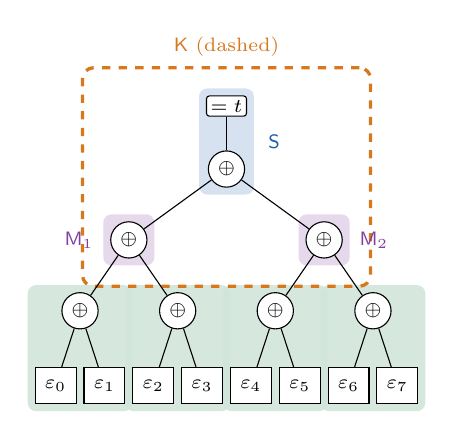
\begin{tikzpicture}
\pic (H) at (0,0) {semtree};
\begin{scope}[on background layer]
\node[region, fill=colS!20, fit=(H-r)(H-g)] (sr) {};
\node[region, fill=colM!22, fit=(H-a)] (m1) {};
\node[region, fill=colM!22, fit=(H-b)] (m2) {};
\foreach \s/\x/\y/\n in {c/l0/l1/1, d/l2/l3/2, e/l4/l5/3, f/l6/l7/4}
  { \node[region, fill=colC!22, fit=(H-\x)(H-\y)(H-\s)] (q\n) {}; }
\node[draw=colK, very thick, dashed, rounded corners=4pt, inner sep=10pt, fit=(H-a)(H-b)(H-r)(H-g)] (kk) {};
\end{scope}
\node[font=\scriptsize, text=colS] at ($(sr.east)+(0.25,0)$) {$\nS$};
\node[font=\scriptsize, text=colM] at ($(m1.west)+(-0.3,0)$) {$\nM_1$};
\node[font=\scriptsize, text=colM] at ($(m2.east)+(0.3,0)$) {$\nM_2$};
\node[font=\scriptsize, text=colK, anchor=south] at (kk.north) {$\nK$ (dashed)};
\end{tikzpicture}
\caption{regions for $N=8$, $d_1=d_2=1$}
\end{subfigure}\hfill
\begin{subfigure}[b]{0.56\textwidth}\centering
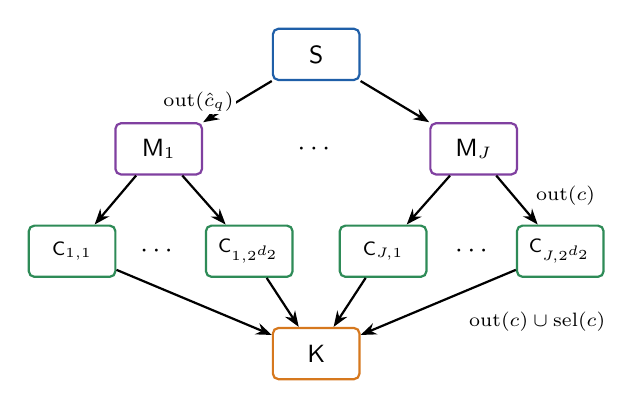
\begin{tikzpicture}
\node[dnode, draw=colS, thick] (S) at (0,3.3) {$\nS$};
\node[dnode, draw=colM, thick] (M1) at (-2.0,2.1) {$\nM_1$};
\node at (0,2.1) {$\cdots$};
\node[dnode, draw=colM, thick] (MB) at (2.0,2.1) {$\nM_{J}$};
\node[dnode, draw=colC, thick, font=\scriptsize] (C11) at (-3.1,0.8) {$\nC_{1,1}$};
\node at (-2.0,0.8) {$\cdots$};
\node[dnode, draw=colC, thick, font=\scriptsize] (C1m) at (-0.85,0.8) {$\nC_{1,2^{d_2}}$};
\node[dnode, draw=colC, thick, font=\scriptsize] (CB1) at (0.85,0.8) {$\nC_{J,1}$};
\node at (2.0,0.8) {$\cdots$};
\node[dnode, draw=colC, thick, font=\scriptsize] (CBm) at (3.1,0.8) {$\nC_{J,2^{d_2}}$};
\node[dnode, draw=colK, thick] (K) at (0,-0.5) {$\nK$};
\draw[sedge] (S) -- node[elab, left] {$\outb(\hat c_q)$} (M1); \draw[sedge] (S) -- (MB);
\draw[sedge] (M1) -- (C11); \draw[sedge] (M1) -- (C1m); \draw[sedge] (MB) -- (CB1); \draw[sedge] (MB) -- (CBm);
\foreach \c in {C11,C1m,CB1,CBm} { \draw[sedge] (\c) -- (K); }
\node[elab, anchor=west] at (2.75,1.5) {$\outb(c)$};
\node[elab, anchor=west] at (1.9,-0.1) {$\outb(c)\cup\selv(c)$};
\end{tikzpicture}
\caption{the DAG}
\end{subfigure}
\caption{Two-stage top-down splitting, \dfam{topdown2:$d_1$:$d_2$}. The top splitter $\nS$
assigns $J=2^{d_1}$ block sub-targets, and each middle splitter $\nM_q$ assigns $2^{d_2}$
subtree sub-targets. The subtrees and the collector $\nK$ (dashed: it holds the whole top
region and the goal) are those of \dfam{topdown:$(d_1+d_2)$}.}
\label{fig:topdown2}
\end{figure}

\begin{table}[htbp]
\centering\small
\begin{tabular}{@{}lllp{0.43\textwidth}@{}}
\toprule
Family & Nodes & Tested & Outcome and lesson \\
\midrule
\dfam{one} & 1 & sandbox, cluster & baseline: 174\,s ($N=2048$), $>$1\,h ($N=4096$) \\
\dfam{split:$K$} & 2 & sandbox, cluster & fast (2.5\,s at $N=2048$ on the cluster), but a cube: flat MiniSat with the same prefix pinned is faster \\
\dfam{tree} & $2N$ & sandbox & joins over variable-disjoint inputs become nested loops: 9{,}206 jobs, timeout at $N=32$ \\
\dfam{block:$B$} & varies & sandbox & enumerating blocks hold workers; with \XSAB{} filtration, intermediate $B$ is best \\
\dfam{topdown:$D$} & $2^D+2$ & sandbox, cluster & independent subtrees; scales to 16--32 workers, then the duplicated splitter overloads the master \\
\dfam{topdown2:$d_1$:$d_2$} & $2^{d_1}+2^{D}+2$ & sandbox, cluster & same subtrees; scales to 207 workers (22.5$\times$ total, 33$\times$ solve) \\
\bottomrule
\end{tabular}
\caption{The DAG families and what each taught us. ``Sandbox'' means one development core;
cluster results are in \cref{sec:results}.}
\label{tab:families}
\end{table}

% ======================================================================
\section{Experimental questions and hypotheses}
\label{sec:questions}
The campaign was organised around five questions. Each hypothesis was stated before the
corresponding runs, and each is answered in \cref{sec:results}.
\begin{enumerate}[label=\textbf{Q\arabic*.}, leftmargin=2.4em]
\item \textbf{Does top-down decomposition beat the one-node formulation on the same hardware?}
      Hypothesis: yes, even on one worker, because many small independent searches are
      cheaper than one large one. This is an \emph{algorithmic} comparison.
\item \textbf{Does the critical-path model, \cref{eq:model}, predict parallel time from a
      one-worker run?} Hypothesis: yes, unless a serial component is missing from the model.
\item \textbf{How does a fixed DAG scale from 1 to 207 workers (strong scaling)?}
      Hypothesis: near-linear until the serial terms ($\Tstart$, $T_K$) dominate.
\item \textbf{Where does time go when scaling stops?} Hypothesis: it is visible in Dagster's
      own logs, without instrumenting Dagster.
\item \textbf{Can the limits be removed without modifying Dagster?} Hypothesis: by choice of
      options and of DAG shape.
\end{enumerate}
\noindent Two questions are \emph{not} answered by this campaign:
\begin{itemize}
\item whether structural distribution beats a matched parallel portfolio of independent
      solvers;
\item how much of the measured overhead is specific to Dagster rather than inherent to the
      decomposition.
\end{itemize}
Both are discussed in \cref{sec:threats}.

% ======================================================================
\section{Experimental setup and methods}
\label{sec:setup}

\subsection{Platform and software}
All results in \cref{sec:results} come from a PBS-managed high-performance computing (HPC)
cluster. Its nodes have 104 cores (Intel Xeon Platinum 8470Q, Sapphire Rapids; two hardware
threads per core, eight NUMA nodes) and 512\,GB of memory. Each MPI rank was bound to one
physical core. Jobs were
submitted through the PBS batch system, and their cost is accounted in \emph{service units}
(SU), which are proportional to cores $\times$ hours.

Dagster was built from the \texttt{AFSAT-Integration} branch (commit \texttt{1c89951},
unmodified). It was launched with Open MPI 4.1.0, one rank per core, using TCP
transport; a comparison with shared-memory transport showed no
difference (\cref{sec:node}). The instances and results lived on a Lustre parallel file
system.

A Python 3.11 harness (standard library only) does the rest:
\begin{itemize}
\item builds each DAG file from the instance metadata;
\item launches Dagster under \texttt{mpirun} and watches for the answer file;
\item ends the MPI session as soon as an answer appears;
\item verifies the answer;
\item records one line of results per run.
\end{itemize}

\paragraph{Provenance of what was executed.}
\begin{itemize}
\item \textbf{Binary.} All 206 runs record the same Dagster build directory, a clone of the
      \texttt{AFSAT-Integration} head at commit \texttt{1c89951}. An older local checkout
      (\texttt{494233b}) that the preparation script once inspected was never used for a
      run. Its SHA-256, captured from that build directory after the campaign, is listed in
      \cref{tab:checksums}. Capturing it at launch time is part of the clean-room procedure
      (\cref{app:repro}).
\item \textbf{Recorded arguments.} 180 runs record the expanded Dagster arguments,
      \opt{-m 4 -e 3 -b 0 -g 2}. The 26 earliest runs predate that field. They record the
      driver flag \opt{--e3}, which in that driver version expanded to
      \opt{-m 4 -e 3 -b 0} and left the master at its default \opt{-g 0}.
\item \textbf{Driver default.} The lower-level launcher's default (\opt{-e 0}) is never used
      in this campaign, because \opt{--e3} replaces it.
\end{itemize}
The environment file loaded by every job is reproduced in \cref{app:repro}.

\subsection{Verification of every answer}
\label{sec:verification}
For every run that returned an answer, the harness reads the reported selector values and
checks that exactly one $x_{i,j}$ is true per episode, which yields the selection $s$. It
then recomputes every summary bit bottom-up through the XOR tree, evaluates \emph{every
clause} of $F$ under the completed assignment, and checks \cref{eq:attack} directly. A run
counts as successful only if all checks pass. A run that produced no answer within its time
limit is recorded as a timeout.

\paragraph{Trust boundary.}
The check is independent of Dagster and MiniSat, but not of the benchmark artefacts: it reads
the generated CNF and the metadata that lists each episode's deltas. Three facts limit the
risk of a shared error:
\begin{itemize}
\item the generator verifies its planted model against every clause before shuffling;
\item its manifest records SHA-256 hashes of the CNF, the metadata and the planted model;
\item the instance files used for analysis match those hashes, and their targets match the
      targets recorded in the campaign's verification messages (\cref{app:evidence}).
\end{itemize}
A second verifier that derives the deltas directly from $N$ and the documented SHA-256 tags,
rather than trusting the stored delta table, would close this gap.

\subsection{What we measured}
\label{sec:metrics}
\begin{itemize}
\item \textbf{Run time $T_P$.} Wall-clock time from launching \texttt{mpirun} with
      $R=P+1$ ranks until the answer file appears. Verification is excluded. $T_1$ is the
      time of the same DAG on one worker ($R=2$). The speedup is $S_P=T_1/T_P$ and the
      efficiency is $E_P=S_P/P$.
\item \textbf{Phases} (\cref{fig:phases}), reconstructed from the master's log of the
      first repeat:
      \begin{itemize}
      \item \emph{start-up} $\Tstart$: from launch until the splitter's job is dispatched,
            plus any time not covered by the log;
      \item \emph{splitter} $T_S$: the top splitter's job;
      \item \emph{subtree phase} $\Tsub$: from the splitter's completion until the last
            subtree finishes (for \dfam{topdown2}, this includes the middle splitters);
      \item \emph{collector} $T_K$: from the collector's dispatch until \emph{its} solution
            arrives.
      \end{itemize}
      The \emph{solve time} is $\Tsolve=T_P-\Tstart$.
\item \textbf{Per-job timing}, from the logs of both sides:
      \begin{itemize}
      \item \emph{compute} $\theta_{\mathrm{comp}}$: from dispatch until the worker reports it has
            finished;
      \item \emph{lag} $\theta_{\mathrm{lag}}$: from the worker's request for new work until the
            master reads it;
      \item \emph{response} $\theta_{\mathrm{resp}}$: from reading the request until the next
            dispatch to that worker.
      \end{itemize}
\item \textbf{Master load $\rho$.} The fraction of the master's loop time spent processing
      messages rather than waiting for them.
\end{itemize}
Scaling runs were repeated three times. Only the first repeat logs at verbosity~3; the
others log nothing, so they time Dagster without logging cost. With fixed node formulas and options, each individual MiniSat job is
deterministic. Parallel repetitions still vary, through process launch, duplicate
allocation, the assignment of jobs to workers, message arrival order, cache state and
contention. Every scaling configuration at $N\ge 8192$ varied by at most 4.7\% between its
fastest and slowest repeat. The median spread over multi-run configurations at $N\le 4096$
was 0.8\%; the largest, 22\%, was in 4-second split runs dominated by start-up jitter.
Medians are descriptive. With two or three repeats per configuration, they do not support
statistical inference. Every individual value is in the archived results
(\cref{app:evidence}).

\subsection{A critical-path performance model}
\label{sec:model}
With one worker per subtree and dedicated cores, the phases of \cref{fig:phases} run in
sequence, and the subtree phase is as long as its slowest subtree. Writing $\Tsub^{\max}$
for the slowest subtree's time and $\Tsub^{\Sigma}$ for the total subtree work,
\begin{equation}
T_P \;\approx\; \Tstart + T_S + \max\!\left(\Tsub^{\max},\ \Tsub^{\Sigma}/P\right) + T_K .
\label{eq:model}
\end{equation}
All terms except $\Tstart$ can be measured on a \emph{one-worker} run, which yields a
prediction for any $P$ before spending supercomputer time. The terms $\Tstart$, $T_S$ and
$T_K$ are serial, so by Amdahl's law they bound the achievable speedup.

\begin{figure}[htbp]
\centering
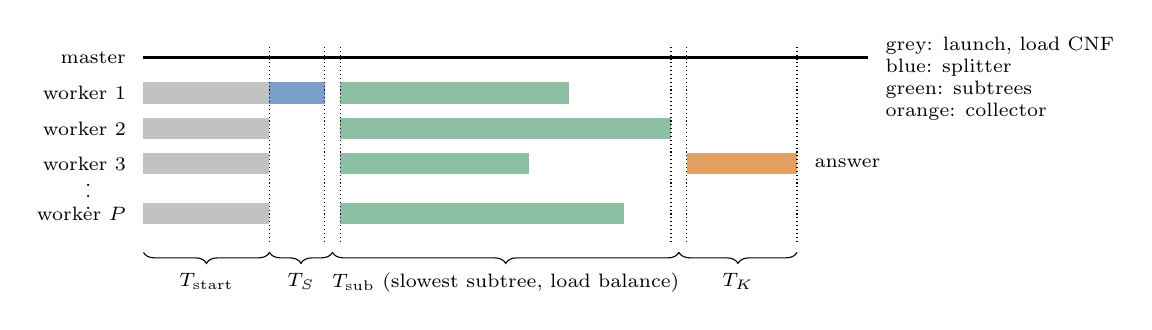
\begin{tikzpicture}[font=\scriptsize, x=1cm, y=0.45cm]
\foreach \w/\y in {master/5, worker 1/4, worker 2/3, worker 3/2, worker $P$/0.6} { \node[anchor=east] at (-0.1,\y) {\w}; }
\node at (-0.7,1.3) {$\vdots$};
\fill[colA!45] (0,4-0.3) rectangle (1.6,4+0.3); \fill[colA!45] (0,3-0.3) rectangle (1.6,3+0.3);
\fill[colA!45] (0,2-0.3) rectangle (1.6,2+0.3); \fill[colA!45] (0,0.6-0.3) rectangle (1.6,0.6+0.3);
\fill[colS!60] (1.6,4-0.3) rectangle (2.3,4+0.3);
\foreach \y/\a/\b in {4/2.5/5.4, 3/2.5/6.7, 2/2.5/4.9, 0.6/2.5/6.1} { \fill[colC!55] (\a,\y-0.3) rectangle (\b,\y+0.3); }
\fill[colK!70] (6.9,2-0.3) rectangle (8.3,2+0.3);
\draw[thick] (0,5) -- (9.2,5);
\foreach \x in {1.6, 2.3, 2.5, 6.7, 6.9, 8.3} { \draw[densely dotted] (\x,-0.2) -- (\x,5.3); }
\draw[decorate,decoration={brace,amplitude=4pt,mirror}] (0,-0.5) -- (1.6,-0.5) node[midway,below=4pt] {$\Tstart$};
\draw[decorate,decoration={brace,amplitude=4pt,mirror}] (1.6,-0.5) -- (2.4,-0.5) node[midway,below=4pt] {$T_S$};
\draw[decorate,decoration={brace,amplitude=4pt,mirror}] (2.4,-0.5) -- (6.8,-0.5) node[midway,below=4pt] {$\Tsub$ (slowest subtree, load balance)};
\draw[decorate,decoration={brace,amplitude=4pt,mirror}] (6.8,-0.5) -- (8.3,-0.5) node[midway,below=4pt] {$T_K$};
\node[anchor=west] at (8.4,2) {answer};
\node[anchor=west, align=left] at (9.3,4.4) {grey: launch, load CNF\\ blue: splitter\\ green: subtrees\\ orange: collector};
\end{tikzpicture}
\caption{The phases of a top-down run, schematically. Start-up (process launch, every rank
loading the CNF) and the collector are serial. The subtree phase is parallel, but no
shorter than its slowest subtree and no shorter than the total subtree work divided by the
number of workers.}
\label{fig:phases}
\end{figure}

% ======================================================================
\section{Results on the HPC cluster}
\label{sec:results}

The experiments ran in the order presented here. Each stage was designed from what the
previous one revealed.

\subsection{Baselines and the one-worker view}
\label{sec:baselines}
\Cref{tab:oneworker} lists times on \emph{one} worker ($R=2$ ranks), which isolate
algorithmic effects from parallel ones:
\begin{itemize}
\item \textbf{Top-down splitting is already faster than one node.} At $N=4096$, one-node
      Dagster did not finish within an hour, while every top-down depth finished within
      four minutes ($\ge 15\times$). The reason is that the solver's effort grows faster
      than linearly in instance size, so many small independent searches cost less than
      one large one.
\item \textbf{The split DAG is the fastest sequential option} (2.5\,s at $N=2048$), but as
      \cref{sec:early} explained, this is the cube effect.
\item \textbf{Under \opt{-g 0}, deeper DAGs got slower on one worker,} even though the
      total subtree work barely changed. The subtree phase exceeded the summed subtree work
      by 33\,s at $N=2048$, depth~8, and by 112\,s at $N=4096$, depth~8. That excess is
      master time spent between jobs, the first sign of the bottleneck in
      \cref{sec:joincheck}.
\end{itemize}

\begin{table}[htbp]
\centering\small
\begin{tabular}{@{}lrrrr@{}}
\toprule
& \multicolumn{2}{c}{$N=2048$} & \multicolumn{2}{c}{$N=4096$} \\
\cmidrule(lr){2-3}\cmidrule(lr){4-5}
DAG (one worker) & \opt{-g 0} & \opt{-g 2} & \opt{-g 0} & \opt{-g 2} \\
\midrule
\dfam{one}        & 174.3 & --- & $>3600$ & --- \\
\dfam{split:8}    & 3.60 & 2.52 & 11.8 & 7.90 \\
\dfam{topdown:3}  & 29.1 & 20.1 & 127.5 & 76.9 \\
\dfam{topdown:5}  & 36.8 & 25.5 & 126.9 & 85.4 \\
\dfam{topdown:7}  & 55.7 & 32.5 & 169.3 & 91.2 \\
\dfam{topdown:8}  & 81.8 & 35.4 & 249.2 & 98.2 \\
\bottomrule
\end{tabular}
\caption{Seconds to a verified attack on one worker. The \opt{-g 2} column skips the
combination check (\cref{sec:joincheck}); a single node has no combinations, so \dfam{one}
was run once.}
\label{tab:oneworker}
\end{table}

\subsection{First parallel runs, and the cost of checking combinations}
\label{sec:joincheck}
We first ran each top-down DAG with one worker per subtree ($R=2^D+1$), using the default
table master. \Cref{eq:model} predicted 8.4, 5.2, 3.3 and 3.1\,s for depths 3, 5, 7 and 8
at $N=2048$:
\begin{itemize}
\item depth~3 on 9 ranks took 8.7\,s, matching the prediction (20$\times$ faster than one
      node);
\item depth~5 on 33 ranks took 17\,s;
\item depths~7 and~8 (129 and 257 ranks) did not finish within 600\,s.
\end{itemize}

\paragraph{Diagnosis.}
The collector $\nK$ has $2^D$ incoming edges, and each message $\mu_i$ on edge $\nC_i\to\nK$
carries $|\mu_i|=W+kQ$ literals. Under \opt{-g 0}, the master's combination search checks
every literal of a candidate message against every literal of the messages already chosen
(\cref{fig:joincheck}). A search that gets through $j$ inputs therefore costs about
$\bigl(\sum_{i\le j}|\mu_i|\bigr)^2/2$ literal comparisons. Until \emph{every} subtree has
reported, each search fails at the first input that has no message yet, and the master
repeats it for \emph{every incoming message}. At $N=2048$ and depth~7, the collector's
inputs total about 33{,}000 literals, so each near-complete search costs about $5\times10^8$
comparisons. With 128 workers reporting at once, the master spends minutes doing nothing
else.

\paragraph{Fix without modifying Dagster.}
In top-down DAGs, the collector's inputs come from different subtrees and share no
variables, so no combination can be inconsistent. The table master without the check
(\opt{-g 2}) is therefore exact here. In general, an inconsistent combination would only
make the receiving job unsatisfiable; it can never produce a wrong model. Because the safety
argument depends on how the graphs are built, we also checked it mechanically. All 55
executed top-down DAG files are acyclic, have exactly one sink (the collector), and give it
pairwise variable-disjoint inputs (\cref{app:evidence}). With \opt{-g 2}
the gap between subtree phase and subtree work vanished (the two now agree to within
0.1\,s), and the one-worker times fell by 31--61\% (\cref{tab:oneworker}).

\begin{figure}[htbp]
\centering
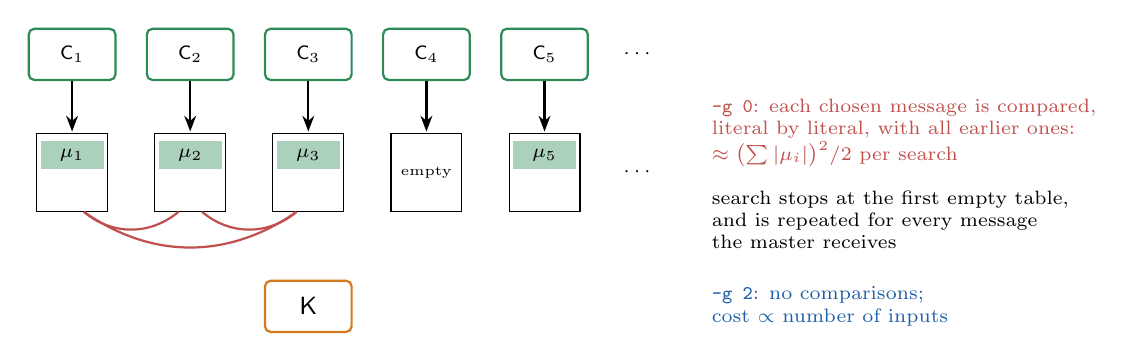
\begin{tikzpicture}[font=\scriptsize]
\foreach \i/\x/\f in {1/0/1, 2/1.5/1, 3/3.0/1, 4/4.5/0, 5/6.0/1} {
  \node[dnode, draw=colC, thick, font=\scriptsize] (c\i) at (\x,2.6) {$\nC_{\i}$};
  \draw[thin] (\x-0.45,0.6) rectangle (\x+0.45,1.6);
  \ifnum\f=1 \fill[colC!40] (\x-0.4,1.15) rectangle (\x+0.4,1.5); \node at (\x,1.32) {$\mu_{\i}$}; \fi
  \draw[sedge] (c\i) -- (\x,1.62);
}
\node at (7.2,2.6) {$\cdots$}; \node at (7.2,1.1) {$\cdots$};
\node[font=\tiny, align=center] at (4.5,1.1) {empty};
\node[dnode, draw=colK, thick] (k) at (3.0,-0.6) {$\nK$};
\foreach \x in {0,1.5} { \draw[colR, thick] (\x+0.15,0.6) to[bend right=40] (\x+1.35,0.6); }
\draw[colR, thick] (0.15,0.6) to[bend right=35] (2.85,0.6);
\node[anchor=west, align=left, text=colR] at (8.0,1.6) {\opt{-g 0}: each chosen message is compared,\\ literal by literal, with all earlier ones:\\ $\approx\bigl(\sum|\mu_i|\bigr)^2/2$ per search};
\node[anchor=west, align=left] at (8.0,0.5) {search stops at the first empty table,\\ and is repeated for every message\\ the master receives};
\node[anchor=west, align=left, text=colS] at (8.0,-0.6) {\opt{-g 2}: no comparisons;\\ cost $\propto$ number of inputs};
\end{tikzpicture}
\caption{Why combining many large messages was expensive. The master keeps one message
table per incoming edge of the collector. Under \opt{-g 0}, each search for a new
combination checks consistency pairwise, literal by literal (red arcs), and the search is
repeated whenever any message arrives. Since the collector's inputs are variable-disjoint,
the check is unnecessary, and \opt{-g 2} removes it.}
\label{fig:joincheck}
\end{figure}

\subsection{One worker per subtree, and over-decomposition on one node}
\label{sec:node}
With \opt{-g 2}, the one-worker-per-subtree runs all succeeded (\cref{tab:wide}). Depth~3
on 9 ranks gave 8.6\,s, i.e.\ 20$\times$ faster than one node at $N=2048$. Larger rank
counts were \emph{slower} than predicted, for two reasons that a dedicated one-node
experiment then separated:
\begin{itemize}
\item \textbf{Start-up grows linearly with the number of ranks.} The one-node DAG on the
      tiny $N=32$ instance solves in milliseconds, so its run time is pure start-up. It
      took 0.9\,s on 2 ranks and 15.7\,s on 104 ranks, about 0.15\,s per rank
      (\cref{fig:startup}). Shared-memory and TCP transport gave identical times. The
      instance plays no role, so the cost lies in process launch and initialisation.
\item \textbf{More subtrees than workers balance the load.} Giving each worker several
      subtrees (depth~7 on 33 ranks, i.e.\ 4 subtrees per worker) was the best
      configuration: 7.7\,s at $N=2048$ (22.6$\times$ faster than one node) and 11.5\,s at
      $N=4096$. That is at least 313 times faster than the one-node run, which was stopped
      at 3{,}600\,s, so the ratio is a lower bound. At $N=4096$ the subtree phase took 4.5\,s, close
      to that run's total subtree work divided by 32 workers (4.3\,s), so the load was
      nearly perfectly balanced. On an otherwise idle node the same work takes 2.75\,s per
      worker; the difference is jobs running slower when every core is busy. More ranks only
      added start-up (\cref{tab:wide}).
\end{itemize}

\begin{table}[htbp]
\centering\small
\begin{tabular}{@{}llrrrr@{}}
\toprule
$N$ & DAG & ranks $R$ & predicted, \eqref{eq:model} & measured & vs.\ one node \\
\midrule
2048 & \dfam{topdown:3} & 9   & 6.0 & 8.57 & 20.3$\times$ \\
2048 & \dfam{topdown:5} & 33  & 3.9 & 9.15 & 19.1$\times$ \\
2048 & \dfam{topdown:7} & 129 & 2.5 & 20.3 & 8.6$\times$ \\
2048 & \dfam{topdown:8} & 257 & 2.4 & 43.9 & 4.0$\times$ \\
\addlinespace
2048 & \dfam{topdown:7} & 33 (one node) & --- & \textbf{7.71} & \textbf{22.6$\times$} \\
2048 & \dfam{topdown:8} & 33 / 65 / 104 & --- & 9.88 / 17.6 / 27.1 & 17.6 / 9.9 / 6.4$\times$ \\
\midrule
4096 & \dfam{topdown:5} & 33  & 10.2 & 15.9 & $>226\times$ \\
4096 & \dfam{topdown:7} & 129 & 5.9 & 23.5 & $>153\times$ \\
4096 & \dfam{topdown:8} & 257 & 4.6 & 48.4 & $>74\times$ \\
\addlinespace
4096 & \dfam{topdown:7} & 33 (one node) & --- & \textbf{11.5} & $\mathbf{>312\times}$ \\
4096 & \dfam{topdown:8} & 33 / 65 / 104 & --- & 13.6 / 21.3 / 30.8 & $>265$ / $>169$ / $>117\times$ \\
\bottomrule
\end{tabular}
\caption{Top-down runs with \opt{-g 2} at $N=2048$ and $4096$ (seconds; medians of 2--3
repeats, which agreed within about 1\%). Rows with one worker per subtree use
$R=2^D+1$ ranks; ``one node'' rows give each worker several subtrees. Speedups at
$N=4096$ are lower bounds, because the one-node run was stopped after 3{,}600\,s.}
\label{tab:wide}
\end{table}

\begin{figure}[htbp]
\centering
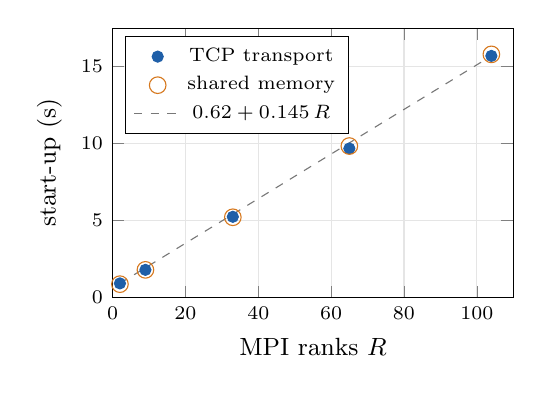
\begin{tikzpicture}
\begin{axis}[width=0.55\textwidth, height=5cm, xlabel={MPI ranks $R$}, ylabel={start-up (s)},
  xmin=0, xmax=110, ymin=0, ymax=17.5, legend pos=north west, legend style={font=\scriptsize},
  tick label style={font=\scriptsize}, label style={font=\small}, grid=major, grid style={gray!20}]
\addplot[only marks, mark=*, colS] coordinates {(2,0.91) (9,1.79) (33,5.24) (65,9.68) (104,15.7)};
\addplot[only marks, mark=o, colK, mark size=3pt] coordinates {(2,0.86) (9,1.79) (33,5.21) (65,9.84) (104,15.8)};
\addplot[colA, dashed, domain=2:104] {0.62+0.145*x};
\legend{TCP transport, shared memory, $0.62+0.145\,R$}
\end{axis}
\end{tikzpicture}
\caption{Start-up versus number of ranks on one cluster node: time to solve a trivial instance
(\XSA{}, $N=32$, one-node DAG), medians of two repeats per transport. The cost is about
0.15\,s per rank and does not depend on the transport.}
\label{fig:startup}
\end{figure}

\subsection{Strong scaling with single-stage splitting, and why it collapsed}
\label{sec:dup}
To make start-up a small fraction of the run, we moved to larger instances ($N=8192$ and
$16384$). We fixed one DAG, \dfam{topdown:9} (512 subtrees), and varied the number of
workers from 1 to 207. The upper rows of \cref{tab:scaling} show that scaling was good up
to 16 workers ($N=8192$) and 32 workers ($N=16384$), but then \emph{reversed}: 207 workers
took longer than 8.

\paragraph{Diagnosis from the logs.}
\Cref{tab:latency} splits each job into the quantities of \cref{sec:metrics}:
\begin{itemize}
\item \textbf{The master's response is never the problem.} Once it read a request, it
      dispatched new work within 3\,ms.
\item \textbf{Requests waited.} The median lag stayed at 0\,ms, but the worst 10\% of
      requests waited up to 175\,s.
\item \textbf{The master was saturated.} At 103 workers it spent 73--87\% of its time
      processing messages, against 3--10\% at 8 workers.
\end{itemize}
Attributing the master's busy time to the messages being processed pinned down the cause.
About 98\% of it went to solutions of the \emph{splitter}:
\begin{itemize}
\item At the start of a run, the splitter's job is the only job, so every idle worker
      received its own copy (\cref{sec:execution}).
\item All the copies produced the same 512-way split at almost the same moment.
\item The master processed each copy in full, restricting it to the splitter's 512
      outgoing edges. That took 0.78--0.97\,s per copy: 25\,s for 32 copies, 89\,s for 103
      and 200\,s for 207.
\item Meanwhile, workers' requests and subtree results queued behind the backlog
      (\cref{fig:backlog}). At 103 workers, the first subtree result was read only at
      $t=90$\,s, and all 512 subtrees then completed within 15\,s.
\end{itemize}
The serial cost is about one second per worker. So adding workers made the run slower.

\begin{table}[htbp]
\centering\small
\begin{tabular}{@{}rrrrrrr@{}}
\toprule
& \multicolumn{2}{c}{lag, 90th percentile} & \multicolumn{2}{c}{master busy $\rho$} & \multicolumn{2}{c}{median job compute} \\
\cmidrule(lr){2-3}\cmidrule(lr){4-5}\cmidrule(lr){6-7}
workers $P$ & $N=8192$ & $16384$ & $8192$ & $16384$ & $8192$ & $16384$ \\
\midrule
8   & 0\,ms   & 0\,ms   & 9.5\% & 3.2\%  & 0.64\,s & 2.4\,s \\
16  & 0\,ms   & 1\,ms   & 27.5\% & 10.9\% & 0.66\,s & 2.5\,s \\
32  & 1\,ms   & 1\,ms   & 57.1\% & 30.2\% & 0.77\,s & 2.9\,s \\
64  & 5.2\,s  & 13.7\,s & 80.5\% & 57.8\% & 1.1\,s & 3.8\,s \\
103 & 79.7\,s & 64.6\,s & 86.8\% & 73.4\% & 1.4\,s & 4.8\,s \\
207 & 169\,s  & 175\,s  & 94.0\% & 88.8\% & 1.7\,s & 5.0\,s \\
\bottomrule
\end{tabular}
\caption{Inside the single-stage (\dfam{topdown:9}) scaling runs, from Dagster's logs. Lag:
time from a worker's request until the master reads it. The master's response after
reading a request never exceeded 3\,ms.}
\label{tab:latency}
\end{table}

\begin{figure}[htbp]
\centering
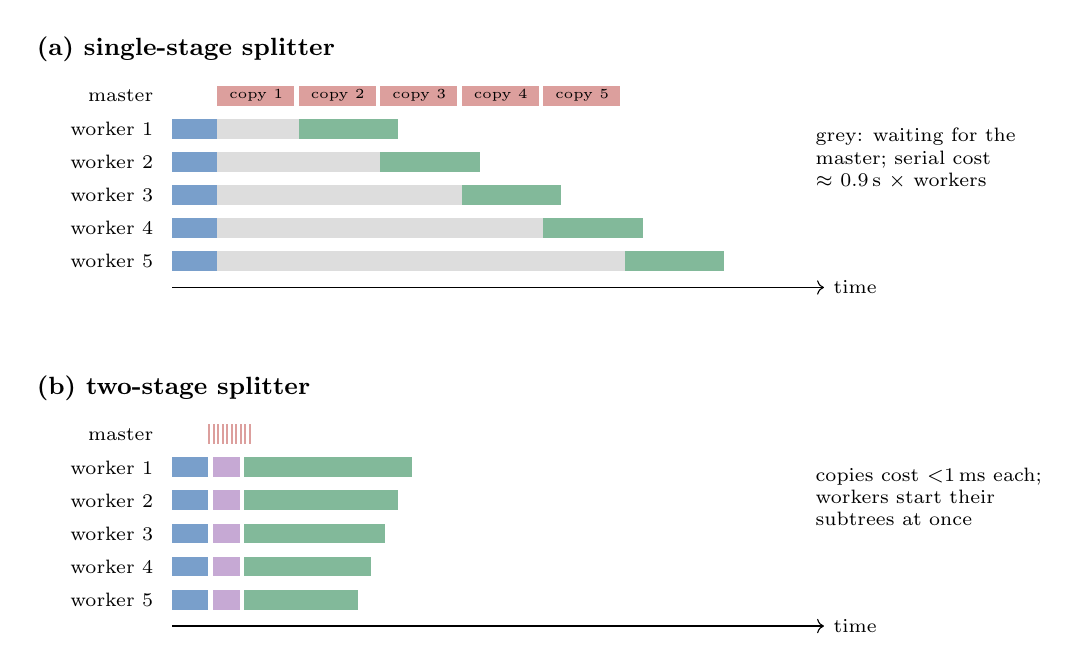
\begin{tikzpicture}[font=\scriptsize, x=1.15cm, y=0.42cm]
\begin{scope}
\node[anchor=west, font=\small\bfseries] at (-1.6,7.4) {(a) single-stage splitter};
\foreach \r/\lab in {6/master, 5/worker 1, 4/worker 2, 3/worker 3, 2/worker 4, 1/worker 5} { \node[anchor=east] at (-0.1,\r) {\lab}; }
\foreach \r in {1,...,5} { \fill[colS!60] (0,\r-0.3) rectangle (0.5,\r+0.3); }
\foreach \k in {1,...,5} {
  \fill[colR!55] (0.5+0.9*\k-0.9,6-0.3) rectangle (0.5+0.9*\k-0.05,6+0.3);
  \node[font=\tiny] at (0.5+0.9*\k-0.47,6) {copy \k};
  \fill[colA!25] (0.5,6-\k-0.3) rectangle (0.5+0.9*\k,6-\k+0.3);
  \fill[colC!60] (0.5+0.9*\k,6-\k-0.3) rectangle (0.5+0.9*\k+1.1,6-\k+0.3);
}
\draw[->] (0,0.2) -- (7.2,0.2) node[right] {time};
\node[align=left, anchor=west] at (7.0,4.1) {grey: waiting for the\\ master; serial cost\\ $\approx$ 0.9\,s $\times$ workers};
\end{scope}
\begin{scope}[yshift=-4.3cm]
\node[anchor=west, font=\small\bfseries] at (-1.6,7.4) {(b) two-stage splitter};
\foreach \r/\lab in {6/master, 5/worker 1, 4/worker 2, 3/worker 3, 2/worker 4, 1/worker 5} { \node[anchor=east] at (-0.1,\r) {\lab}; }
\foreach \r in {1,...,5} { \fill[colS!60] (0,\r-0.3) rectangle (0.4,\r+0.3); \fill[colM!45] (0.45,\r-0.3) rectangle (0.75,\r+0.3); \fill[colC!60] (0.8,\r-0.3) rectangle (1.9+0.15*\r,\r+0.3); }
\foreach \k in {0,...,9} { \fill[colR!55] (0.4+0.05*\k,6-0.3) rectangle (0.42+0.05*\k,6+0.3); }
\draw[->] (0,0.2) -- (7.2,0.2) node[right] {time};
\node[align=left, anchor=west] at (7.0,4.1) {copies cost $<$1\,ms each;\\ workers start their\\ subtrees at once};
\end{scope}
\end{tikzpicture}
\caption{The duplicate-splitter backlog, schematically (not to scale). Blue: copies of the
top splitter; purple: middle splitters; green: subtrees; red: the master processing a
splitter solution. (a) With one 512-way splitter, every idle worker runs a copy, and the
master processes the identical solutions one by one, at about 0.9\,s each on the cluster. Workers
receive their first subtree only after their copy has been processed. (b) With two-stage
splitting each copy is small, and the backlog disappears.}
\label{fig:backlog}
\end{figure}

\subsection{Two-stage splitting removes the bottleneck}
\label{sec:twostage}
The two-stage family (\cref{sec:topdown2}) keeps the subtrees and the collector, but
replaces the single 512-way split by a 16-way split followed by sixteen 32-way splits. Its
effect on the master was measured first on one worker at $N=4096$, in the sandbox:
\begin{itemize}
\item \textbf{Per splitter solution,} the master's processing time fell from 1{,}257\,ms
      (single-stage) to 0.22\,ms for the top splitter and about 1\,ms for a middle
      splitter (at most 1.9\,ms). A subtree solution costs 0.14\,ms in both DAGs.
\item \textbf{The search work was unchanged:} 194\,s against 193\,s, both answers verified.
\end{itemize}

On the cluster the master's load fell from 73--94\% to 7--20\% at 103--207 workers. Some 100--200
copies of the top splitter now cost it 12--26\,ms \emph{in total}, against 89--200\,s
before. The 90th-percentile lag stayed below 70\,ms throughout.

The scaling curve no longer reverses (\cref{fig:scaling}, \cref{tab:scaling}):
\begin{itemize}
\item \textbf{$N=16384$:} the run time falls monotonically from 1{,}447.6\,s on one worker to
      64.3\,s on 207 workers (63.0 and 65.6\,s in the two repeats). That is a speedup of
      22.5 with efficiency $E_{207}=10.9\%$, and 33.1 with efficiency 16.0\% for the solve
      phase. The run consumed 9.2 times the worker core-seconds of the one-worker run: it
      trades aggregate compute for time-to-solution.
\item \textbf{$N=8192$:} the total reaches 27.8\,s at 32 workers (14$\times$), then stays
      near 30\,s, because start-up grows while the solve time keeps falling (28.5$\times$
      at 207 workers).
\end{itemize}

\begin{figure}[htbp]
\centering
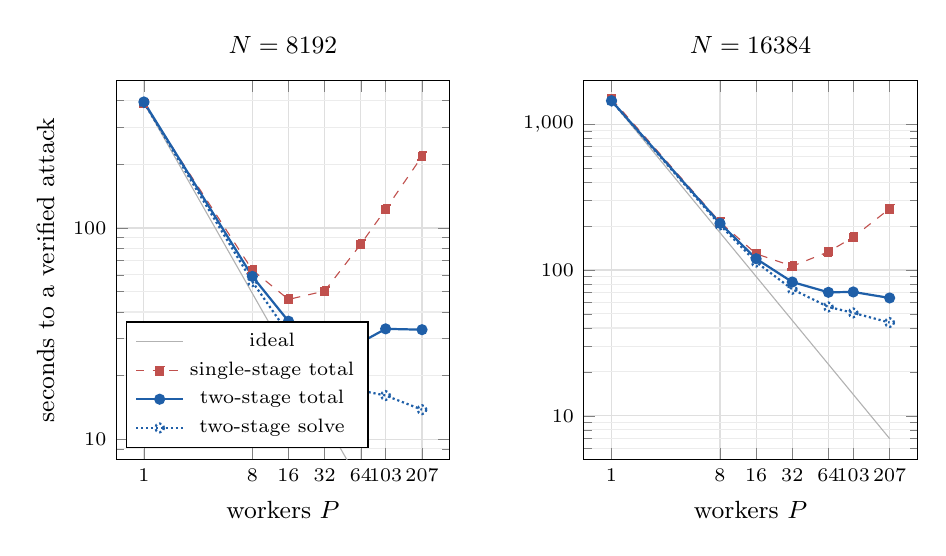
\begin{tikzpicture}
\begin{groupplot}[group style={group size=2 by 1, horizontal sep=1.7cm},
  width=0.48\textwidth, height=6.4cm, xmode=log, ymode=log, log basis x=2,
  xtick={1,8,16,32,64,103,207}, xticklabels={1,8,16,32,64,103,207},
  xlabel={workers $P$}, grid=both, grid style={gray!15}, major grid style={gray!25},
  tick label style={font=\scriptsize}, label style={font=\small}, title style={font=\small},
  log ticks with fixed point, legend style={font=\scriptsize, at={(0.03,0.03)}, anchor=south west}]
\nextgroupplot[title={$N=8192$}, ylabel={seconds to a verified attack}, ymin=8, ymax=500]
\addplot[gray!60, thin, domain=1:207, samples=2] {392.3/x};
\addplot[colR, dashed, mark=square*, mark size=1.6pt] coordinates {(1,388.3) (8,63.2) (16,45.9) (32,50.3) (64,83.8) (103,122.5) (207,218.2)};
\addplot[colS, thick, mark=*, mark size=1.6pt] coordinates {(1,394.9) (8,59.0) (16,36.2) (32,27.8) (64,28.7) (103,33.3) (207,33.0)};
\addplot[colS, densely dotted, thick, mark=o, mark size=1.6pt] coordinates {(1,392.3) (8,55.7) (16,31.6) (32,21.1) (64,17.0) (103,16.1) (207,13.8)};
\legend{ideal, single-stage total, two-stage total, two-stage solve}
\nextgroupplot[title={$N=16384$}, ymin=5, ymax=2000]
\addplot[gray!60, thin, domain=1:207, samples=2] {1443.4/x};
\addplot[colR, dashed, mark=square*, mark size=1.6pt] coordinates {(1,1494.7) (8,213.1) (16,129.2) (32,106.2) (64,133.3) (103,168.0) (207,263.3)};
\addplot[colS, thick, mark=*, mark size=1.6pt] coordinates {(1,1447.6) (8,209.1) (16,119.5) (32,82.7) (64,70.3) (103,70.7) (207,64.3)};
\addplot[colS, densely dotted, thick, mark=o, mark size=1.6pt] coordinates {(1,1443.4) (8,203.8) (16,113.3) (32,73.8) (64,55.8) (103,50.8) (207,43.6)};
\end{groupplot}
\end{tikzpicture}
\caption{Strong scaling on the cluster with unmodified Dagster (\opt{-m 4 -e 3 -g 2}), both instances
with 512 subtrees. Red: single-stage splitting (\dfam{topdown:9}). Blue: two-stage
splitting (\dfam{topdown2:4:5}), total and solve time (total minus start-up). Grey: ideal
scaling of the one-worker solve time. 103 workers fill one node (104 ranks); 207 workers
fill two. Medians of 2--3 repeats.}
\label{fig:scaling}

\vspace{6mm}
\small
\setlength{\tabcolsep}{4.5pt}
\begin{tabular}{@{}rrrrrrrr@{}}
\toprule
& single-stage & \multicolumn{6}{c}{two-stage (\dfam{topdown2:4:5})} \\
\cmidrule(lr){2-2}\cmidrule(l){3-8}
$P$ & total & total (min--max) & $S_P$ & $E_P$ & $S_P^{\mathrm{solve}}$ & $E_P^{\mathrm{solve}}$ & core-s ratio \\
\midrule
\multicolumn{8}{@{}l}{$N=8192$}\\
1   & 388.3 & 394.9 & 1.00 & 100\% & 1.00 & 100\% & 1.00 \\
8   & 63.2  & 59.0 (58.9--59.6) & 6.70 & 84\% & 7.05 & 88\% & 1.20 \\
16  & 45.9  & 36.2 (36.2--36.3) & 10.9 & 68\% & 12.4 & 78\% & 1.47 \\
32  & 50.3  & 27.8 (27.8--28.0) & 14.2 & 44\% & 18.6 & 58\% & 2.26 \\
64  & 83.8  & 28.7 (28.1--29.0) & 13.7 & 21\% & 23.1 & 36\% & 4.66 \\
103 & 122.5 & 33.3 (32.2--33.6) & 11.8 & 11\% & 24.4 & 24\% & 8.70 \\
207 & 218.2 & 33.0 (32.2--33.8) & 12.0 & 5.8\% & 28.5 & 14\% & 17.3 \\
\addlinespace
\multicolumn{8}{@{}l}{$N=16384$}\\
1   & 1494.7 & 1447.6 & 1.00 & 100\% & 1.00 & 100\% & 1.00 \\
8   & 213.1 & 209.1 (209.0--209.1) & 6.92 & 87\% & 7.08 & 89\% & 1.16 \\
16  & 129.2 & 119.5 (119.4--119.7) & 12.1 & 76\% & 12.7 & 80\% & 1.32 \\
32  & 106.2 & 82.7 (82.6--82.7)   & 17.5 & 55\% & 19.6 & 61\% & 1.83 \\
64  & 133.3 & 70.3 (70.2--70.8)   & 20.6 & 32\% & 25.9 & 40\% & 3.11 \\
103 & 168.0 & 70.7 (70.3--70.9)   & 20.5 & 20\% & 28.4 & 28\% & 5.03 \\
207 & 263.3 & \textbf{64.3} (63.0--65.6) & \textbf{22.5} & \textbf{10.9\%} & \textbf{33.1} & \textbf{16.0\%} & 9.19 \\
\bottomrule
\end{tabular}
\captionof{table}{Strong-scaling data behind \cref{fig:scaling} (seconds; median, with the
range over 3 repeats, or 2 at 207 workers). For the two-stage DAG: $S_P=T_1/T_P$ and
$E_P=S_P/P$; ``solve'' excludes start-up; the core-second ratio is $P\,T_P/T_1$. Including
the master rank changes it by under 2\%.}
\label{tab:scaling}
\end{figure}

\paragraph{What limits the two-stage curve.}
\Cref{fig:breakdown} splits the $N=16384$ runs into phases. At 207 workers the 64\,s divide
roughly into thirds:
\begin{itemize}
\item \textbf{start-up, 20.7\,s,} which grows with the number of ranks;
\item \textbf{the subtree phase, 20.3\,s,} against an ideal of 6.9\,s (1{,}424\,s of
      one-worker subtree work divided by 207). Jobs run slower on fully loaded nodes:
      the median subtree job rises from 2.2\,s to 2.7\,s and the 90th percentile from
      5.2\,s to 11.0\,s, pointing to shared memory bandwidth. The slowest subtrees also
      form a tail;
\item \textbf{the collector, 23.2\,s,} a serial step whose cost grows about four-fold per
      doubling of $N$: 1.0\,s, 4.9\,s and 19.4\,s at $N=4096$, 8192 and 16384 on one
      worker. Its input of $\approx NQ$ selector literals grows by a factor of 2.12 per
      doubling, so the fitted exponents relative to input size are 2.1 and 1.8. This is
      \emph{consistent with} quadratic behaviour, but three points cannot establish it;
      profiling and a finer size sweep are needed.
\end{itemize}

\begin{figure}[htbp]
\centering
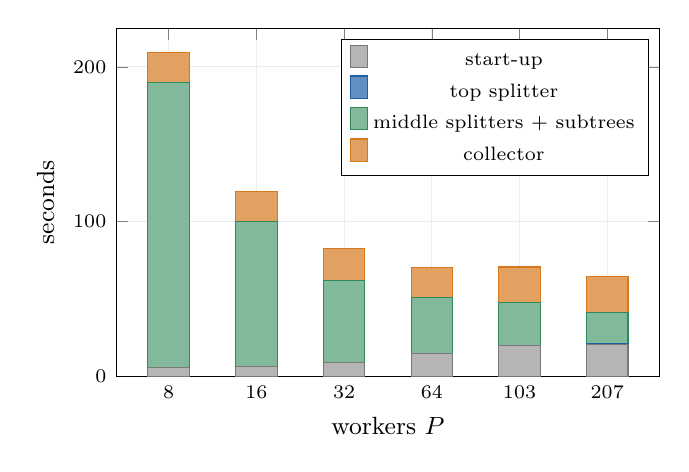
\begin{tikzpicture}
\begin{axis}[ybar stacked, bar width=15pt, width=0.7\textwidth, height=6cm,
  symbolic x coords={8,16,32,64,103,207}, xtick=data, xlabel={workers $P$}, ylabel={seconds},
  ymin=0, ymax=225, legend style={font=\scriptsize, at={(0.98,0.97)}, anchor=north east},
  tick label style={font=\scriptsize}, label style={font=\small}, enlarge x limits=0.12,
  nodes near coords={}, grid=major, grid style={gray!15}]
\addplot[fill=colA!55, draw=colA] coordinates {(8,5.32) (16,6.21) (32,8.89) (64,14.43) (103,19.81) (207,20.69)};
\addplot[fill=colS!70, draw=colS] coordinates {(8,0.10) (16,0.09) (32,0.10) (64,0.12) (103,0.14) (207,0.14)};
\addplot[fill=colC!60, draw=colC] coordinates {(8,184.2) (16,93.7) (32,53.1) (64,36.3) (103,27.4) (207,20.3)};
\addplot[fill=colK!70, draw=colK] coordinates {(8,19.4) (16,19.4) (32,20.5) (64,19.5) (103,23.2) (207,23.2)};
\legend{start-up, top splitter, middle splitters + subtrees, collector}
\end{axis}
\end{tikzpicture}
\caption{Where the time goes: two-stage splitting at $N=16384$, reconstructed from Dagster's
logs (first repeat). The parallel subtree phase shrinks with $P$; the serial start-up and
collector do not.}
\label{fig:breakdown}
\end{figure}

\subsection{A measurement pitfall: whose solution is it?}
\label{sec:pitfall}
Our first phase analysis took the first solution the master received after dispatching the
collector to be the collector's. With duplicate jobs, however, a leftover copy of a
subtree often reports in between. The collector's real solve time (19--23\,s at
$N=16384$) was then silently counted as start-up. Matching the collector's solution to the
worker that received the collector's job fixed this. All phase figures in this report use
the corrected attribution. Totals are unaffected; only the split between start-up and
solve time changed.

\subsection{Run inventory, correctness and cost}
\label{sec:correctness}
\Cref{tab:inventory} accounts for every one of the 206 cluster runs:
\begin{itemize}
\item 203 returned an attack, and every one passed the full verification of
      \cref{sec:verification};
\item 3 were censored by their time limit: the one-node baseline at $N=4096$ (3{,}600\,s),
      and depths~7 and~8 under \opt{-g 0} (600\,s);
\item there were no launch failures and no invalid models.
\end{itemize}
Before the cluster campaign, a separate correctness campaign in the sandbox had run 144 Dagster
configurations on 18 instances (including generic tree-decomposition DAGs) without a wrong
answer.

\begin{table}[htbp]
\centering\small
\setlength{\tabcolsep}{3pt}
\begin{tabular}{@{}llllrrrrr@{}}
\toprule
PBS job & experiment (bundle) & $N$ & DAGs & ranks & reps & runs & verified & censored \\
\midrule
181048154 & smoke (v2) & 32 & one, split, td1--2 & 2--5 & 1 & 6 & 6 & 0 \\
181049118 & one worker, \opt{-g 0} (v2) & 2048, 4096 & one, split, td3--8 & 2 & 1 & 12 & 11 & 1 \\
181049119 & wide, \opt{-g 0} (v2) & 2048 & split, td3--8 & 3--257 & 1--2 & 8 & 6 & 2 \\
181060407 & smoke (v3) & 32 & one, split, td1--2 & 2--5 & 1 & 6 & 6 & 0 \\
181060605 & one worker (v3) & 2048, 4096 & split, td3--8 & 2 & 1 & 10 & 10 & 0 \\
181060606 & wide (v3) & 2048, 4096 & split, td3--8 & 3--257 & 3 & 24 & 24 & 0 \\
181061721 & one node (v4) & 32, 2048, 4096 & one, td5--8 & 2--104 & 2 & 68 & 68 & 0 \\
181063449 & scaling ref.\ (v5) & 8192, 16384 & td9 & 2 & 1 & 2 & 2 & 0 \\
181064188 & scaling (v5) & 8192, 16384 & td9 & 9--104 & 3 & 30 & 30 & 0 \\
181064189 & scaling, 2 nodes (v5) & 8192, 16384 & td9 & 208 & 2 & 4 & 4 & 0 \\
181115773 & scaling ref.\ (v6) & 8192, 16384 & td2:4:5 & 2 & 1 & 2 & 2 & 0 \\
181115774 & scaling (v6) & 8192, 16384 & td2:4:5 & 9--104 & 3 & 30 & 30 & 0 \\
181115775 & scaling, 2 nodes (v6) & 8192, 16384 & td2:4:5 & 208 & 2 & 4 & 4 & 0 \\
\midrule
& & & & & & \textbf{206} & \textbf{203} & \textbf{3} \\
\bottomrule
\end{tabular}
\caption{Every run of the campaign, by PBS job. ``td$D$'' abbreviates \dfam{topdown:$D$}, and the
bundle version gives the scripts that were submitted; the scripts in \texttt{hpc/} of the
repository are version~6 with site settings removed. Regenerated from the raw results by
\texttt{derive.py} (\texttt{inventory.csv}, \cref{app:evidence}).}
\label{tab:inventory}
\end{table}

\paragraph{Cost.}
PBS reported service units for 12 of the 13 jobs, 1{,}052\,SU in all:
\begin{itemize}
\item small jobs: the first smoke test 0.07\,SU, and the one-worker jobs 12.6\,SU and
      1.4\,SU;
\item the two wide jobs: 317.7\,SU (it hit its walltime) and 109.4\,SU;
\item the one-node experiment: 64.7\,SU;
\item the single-stage scaling jobs: 14.8\,SU, 211.1\,SU and 123.4\,SU;
\item the two-stage scaling jobs: 13.7\,SU, 145.6\,SU and 37.2\,SU.
\end{itemize}
The second smoke test's figure was not captured. In core-seconds, the headline run at 207
workers used 9.2 times the work of the one-worker run (\cref{tab:scaling}).

% ======================================================================
\section{Threats to validity}
\label{sec:threats}
\paragraph{Missing comparisons.}
\begin{itemize}
\item \textbf{No matched portfolio.} No MiniSat portfolio (independent solvers with
      different seeds on the same cores, first verified model wins) was run on the cluster for these
      instances. Without it, the report shows that one DAG scales, not that structural
      distribution beats ordinary parallel SAT. Sequential MiniSat at $N=2048$ varied from
      35\,s to 156\,s across three seeds, so a portfolio would profit from the heavy tail.
\item \textbf{No direct dispatcher.} No implementation of the same top-down computation
      without Dagster was run: choose sub-targets, solve subtrees as independent jobs,
      concatenate, verify. So we cannot separate Dagster's overhead from the
      decomposition's.
\end{itemize}

\paragraph{The benchmark (construct validity).}
\XSA{} is solution-dense and admits a sequential shortcut, and it is not a protocol model
(\cref{sec:boundaries}). The results speak to orchestration and scaling, not to search
power, and they do not automatically transfer to protocol encodings.

\paragraph{Model assumptions.}
The acceptance predictor, \cref{eq:pacc}, is a random-XOR approximation. It was confirmed
empirically for every executed configuration, not proven.

\paragraph{Measurement.}
\begin{itemize}
\item Medians come from two or three repeats; they are descriptive.
\item Phase timings come from the first, logged, repeat, whose totals agreed with the
      unlogged repeats to within a few per cent.
\item Phases are reconstructed from log lines, using attribution rules that were themselves
      corrected once (\cref{sec:pitfall}).
\item In two-node runs, timestamps come from two hosts' clocks.
\item Wall time includes the harness's polling granularity (50\,ms).
\end{itemize}

\paragraph{External validity.}
One platform (one cluster's Sapphire Rapids nodes), one solver engine (MiniSat), one MPI
configuration (Open MPI 4.1.0 over TCP), and at most two nodes.

\paragraph{Provenance gaps.}
The Dagster binary's SHA-256, the instance checksums for $N\ge 8192$, the compiler,
operating system and CPU configuration were captured after the campaign. They come from the
same build directory, instance files and node type, not from records written at launch. Still
not recorded:
\begin{itemize}
\item compiler flags and the glog and CUDD versions;
\item resource limits, the NUMA balancing policy and page-cache state;
\item the service units of the second smoke test.
\end{itemize}
Hyper-threading was enabled at the operating-system level, two hardware threads per core.
Ranks were bound one per physical core, so no two ranks shared a core.

\paragraph{Sandbox-only results.}
These come from one development core, not from the cluster, and are qualitative:
\begin{itemize}
\item the early families (\cref{sec:early});
\item the \XSAB{} measurements (\cref{sec:xsab});
\item the single-stage versus two-stage splitter-cost comparison;
\item the refinement result cited in future work.
\end{itemize}


\label{sec:rules}
The experiments condense into ten rules. Each one is backed by a measurement in this report.
\begin{enumerate}[label=\textbf{R\arabic*.}, leftmargin=2.6em]
\item \textbf{Every join must filter.} A node with several inputs runs one job per
      consistent combination of input messages. If the inputs share no variables, every
      combination is consistent and the node becomes a nested loop (\dfam{tree}: 9{,}206
      jobs and a timeout at $N=32$).
\item \textbf{Single-shot only above the acceptance floor.} Under \opt{-e 3} a producer
      offers one message, so every consumer must accept it with probability $\approx 1$.
      Choose the depth with \cref{eq:pacc}; at $N=32$, depth~3 gave $\Pall=0.85\%$.
\item \textbf{Never let enumerating nodes outnumber workers.} A node that streams
      solutions holds its worker indefinitely, and the others starve (\dfam{block:8}: 2
      jobs in 100\,s).
\item \textbf{Compare with the flat solver given the same knowledge.} A pinned prefix (the
      split's cube) or a filtration (\XSAB{}'s strategy) helps a single solver as much as
      it helps the DAG.
\item \textbf{Coarsen until a job's work exceeds its overhead.} Fusing the lower levels of
      a tree into blocks cut \XSAB{}'s jobs from 4{,}081 to 25.
\item \textbf{Skip the combination check when inputs are variable-disjoint.} The table
      master's check costs $\approx(\sum|\mu_i|)^2/2$ per search and is repeated per
      message; \opt{-g 2} is exact when inputs cannot conflict (\cref{sec:joincheck}).
\item \textbf{Over-decompose.} Several subtrees per worker balance the load: depth~7 on 33
      ranks beat one subtree per worker on 129 ranks (\cref{sec:node}).
\item \textbf{Keep any job that may be duplicated cheap to report.} The only initial job is
      copied to every idle worker, and the master processes every copy's solution in full.
      Stage wide splits (\cref{sec:twostage}).
\item \textbf{Predict before you spend.} A one-worker run plus \cref{eq:model} predicts
      the parallel time. Disagreements point at a bottleneck, which the logs can locate,
      provided each solution is attributed to the worker that produced it
      (\cref{sec:pitfall}).
\item \textbf{Size the rank count to the work.} Start-up costs $\approx0.15$\,s per rank,
      and the collector is serial; by Amdahl's law, both cap useful parallelism
      (\cref{fig:breakdown}).
\end{enumerate}

% ======================================================================
\section{Conclusions and future work}
\label{sec:conclusions}

\paragraph{Headline, and its limits.}
For deterministic \XSA{} instances and a fixed two-stage top-down DAG, unmodified Dagster
achieved a 22.5-fold strong-scaling speedup from one to 207 MiniSat workers on an HPC cluster
($N=16384$: 1{,}447.6\,s to 64.3\,s). Efficiency was 10.9\%, or 16.0\% for the solve phase,
and the run used 9.2 times the worker core-seconds. Every returned attack was independently
verified.

This result does \emph{not} show:
\begin{itemize}
\item that Dagster is the fastest way to solve \XSA{}: a sequential cube is faster;
\item that top-down decomposition beats a matched portfolio, which was not run;
\item that the result transfers automatically to real protocol encodings;
\item that the acceptance predictor is a guarantee;
\item that 207 workers use compute efficiently.
\end{itemize}

\paragraph{Conclusions about the benchmark.}
\begin{enumerate}
\item \textbf{The natural bottom-up decomposition is operationally poor.} Its joins do not
      filter, and they turn into nested loops.
\item \textbf{Plentiful solutions make cube controls unusually strong.} Fixing almost every
      choice leaves an easy residue.
\item \textbf{Top-down sub-targets create independent, satisfiable sub-problems.} By the
      algebra of XOR, any split of the target is valid, and above the acceptance floor every
      piece succeeds. Even on one worker this beats the one-node formulation, which is an
      algorithmic gain.
\item \textbf{\XSA{} suits orchestration and scaling studies,} not claims of algorithmic
      superiority.
\end{enumerate}

\paragraph{Conclusions about Dagster.}
\begin{enumerate}
\item \textbf{Multi-input nodes over unfiltered inputs are dangerous:} one job per
      combination.
\item \textbf{The default consistency check can dominate wide joins over variable-disjoint
      inputs.} Disabling it (\opt{-g 2}) is exact when disjointness is verified.
\item \textbf{Eager duplication of the only pending job, plus serial processing of every
      duplicate's result, can overload the single master.} Staging a wide splitter reduces
      the cost of each duplicate from about a second to milliseconds.
\item \textbf{Start-up and the final collector are then the serial limits,} together with
      slower jobs on fully loaded nodes.
\item \textbf{Dagster's own logs were sufficient} to diagnose every one of these mechanisms,
      provided each solution is attributed to the worker that produced it.
\end{enumerate}

\paragraph{Future work, tier 1: complete the evidence for this report.}
\begin{enumerate}
\item Run an equal-core MiniSat portfolio on the same instances and limits.
\item Run a direct, non-Dagster implementation of the same top-down decomposition. Together
      with the portfolio, this gives a four-way comparison: flat MiniSat, portfolio, direct
      dispatcher, Dagster.
\item Profile the collector. Then test linear, $n\log n$ and quadratic models on a finer
      size sweep.
\item Record provenance at launch rather than afterwards: the binary's SHA-256,
      compiler flags, library versions and resource limits. Also record total CPU and
      memory per run (\cref{app:repro}).
\end{enumerate}

\paragraph{Tier 2: improve Dagster (suggestions for upstream, not applied here).}
\begin{enumerate}
\item Suppress identical results before projecting them onto outgoing edges.
\item Avoid eager duplication of the only pending job, or cap duplicates per node.
\item Make the consistency check incremental, or skip it automatically when incoming
      variable sets are pairwise disjoint.
\item Support hierarchical collectors.
\item Load per-node formulas instead of the full CNF on every rank.
\item Emit structured, machine-readable events that separate launch, formula load and
      solver initialisation, and report the master's queue depth.
\end{enumerate}

\paragraph{Tier 3: generalise beyond \XSA{}.}
\begin{enumerate}
\item Scale \XSAB{} with filtration, keeping the same-knowledge flat control (rule~R4).
\item Test scarce-solution problems without a trivial residue.
\item Test a concrete bounded protocol encoding from BMC or
      CBMC~\cite{biere1999bmc,clarke2004cbmc}.
\item Test memory-bound cases where one-node execution is infeasible.
\item Adapt the decomposition from telemetry, re-splitting slow subtrees. In the sandbox,
      three refinement rounds more than halved the slowest subtree, from 6.45\,s to 2.97\,s.
\item Run beyond two nodes, measure weak scaling, and compare worker engines (MiniSat,
      CryptoMiniSat, CaDiCaL, Kissat) where integration permits.
\end{enumerate}

% ======================================================================
\appendix
\section{Table of notation}
\label{app:notation}
\small
\begin{longtable}{@{}p{0.2\textwidth}p{0.62\textwidth}p{0.1\textwidth}@{}}
\toprule
Symbol & Meaning & Section \\
\midrule
\endhead
\multicolumn{3}{@{}l}{\emph{Satisfiability}}\\
$x$, $\neg x$ & a Boolean variable and its negation & \ref{sec:background} \\
$\ell$ & a literal: a variable or its negation & \ref{sec:background} \\
$C$ & a clause: a disjunction of literals & \ref{sec:background} \\
$F$, $|F|$ & a CNF formula (conjunction of clauses) and its number of clauses & \ref{sec:background} \\
$V$, $|V|$ & the set of variables of $F$ and its size & \ref{sec:background} \\
$\alpha$, $\alpha\models F$ & an assignment; $\alpha$ satisfies $F$ & \ref{sec:background} \\
$\oplus$ & exclusive-or (XOR), bitwise on words & \ref{sec:encodings} \\
\addlinespace
\multicolumn{3}{@{}l}{\emph{Dagster}}\\
$G=(U,E)$ & a Dagster DAG with node set $U$ and edge set $E$ & \ref{sec:dagster} \\
$u$, $v$; $e=(u,v)$ & DAG nodes; a directed edge from $u$ to $v$ & \ref{sec:dagster} \\
$F_u$ & the clauses held by node $u$ & \ref{sec:dagster} \\
$I_e$ & the interface variables carried by edge $e$ & \ref{sec:dagster} \\
$\mu$, $|\mu|$ & a message (an assignment of $I_e$) and its number of literals & \ref{sec:dagster} \\
$n_v$ & the number of incoming edges of node $v$ & \ref{sec:dagster} \\
$\alpha_{\mathrm{in}}$ & a job's input: the union of one message per incoming edge & \ref{sec:dagster} \\
$\beta$ & a solution found by a job & \ref{sec:dagster} \\
$R$, $P=R-1$ & number of MPI ranks; number of workers & \ref{sec:execution} \\
\addlinespace
\multicolumn{3}{@{}l}{\emph{The benchmark}}\\
$N$ & number of episodes (sessions); the single scale parameter & \ref{sec:xsa-formal} \\
$Q$, $W$ & transcripts per episode; bit width of deltas and summaries, \eqref{eq:qw} & \ref{sec:xsa-formal} \\
$i$, $j$ & episode index ($0\le i<N$); transcript index ($0\le j<Q$) & \ref{sec:xsa-formal} \\
$\delta_{i,j}$ & the $W$-bit delta of transcript $j$ in episode $i$ & \ref{sec:xsa-formal} \\
$s=(s_0,\dots,s_{N-1})$ & a selection: one transcript per episode & \ref{sec:xsa-formal} \\
$t$ & the target fingerprint ($W$ bits) & \ref{sec:xsa-formal} \\
$\widehat{\lambda}(k)$ & random-XOR predictor: expected number of $k$-episode selections hitting a fixed target, $Q^k/2^W$ (the hat marks a model quantity) & \ref{sec:xsa-formal} \\
$\varepsilon_i$, $\gamma$ & episode node $i$; the goal node & \ref{sec:encoding} \\
$h$ & level of a join node (a level-$h$ join covers $2^{h+1}$ episodes) & \ref{sec:encoding} \\
$\outb(n)$, $\lv(n)$, $\selv(n)$ & summary bits of semantic node $n$; its episodes; their selectors & \ref{sec:encoding} \\
$x_{i,j}$, $y_{n,b}$ & selector variable; summary bit $b$ ($0\le b<W$) of node $n$ & \ref{sec:encoding} \\
$m$, $\omega$ & \XSAB{}: $N=2^m$ episodes, $Q=2^\omega$ choices, $W=\omega(m+1)$ & \ref{sec:xsab} \\
\addlinespace
\multicolumn{3}{@{}l}{\emph{Decompositions}}\\
$K$; $\nA$, $\nB$ & \dfam{split}: residual block size; its two DAG nodes & \ref{sec:early} \\
$B$ & \dfam{block}: maximum episodes per fused block & \ref{sec:early} \\
$D$, $k=N/2^D$ & top-down depth; episodes per subtree & \ref{sec:topdown} \\
$c_i$, $\mathcal{T}_D$ & subtree roots at depth $D$; the joins above them (top region) & \ref{sec:topdown} \\
$\nS$, $\nC_i$, $\nK$ & splitter, subtree and collector nodes & \ref{sec:topdown} \\
$\tau_i$ & the sub-target of subtree $i$ & \ref{sec:topdown} \\
$\pacc(k)$, $\Pall(D)$ & probability that one subtree / all subtrees reach their sub-targets, \eqref{eq:pacc} & \ref{sec:topdown} \\
$\kappa$; $\eta$ & keyed variant: the whole split; bounded variant: free bits per sub-target & \ref{sec:topdown} \\
$d_1$, $d_2$ & \dfam{topdown2}: depths of the two splitting stages, $D=d_1+d_2$ & \ref{sec:topdown2} \\
$J=2^{d_1}$, $q$, $\hat c_q$ & number of blocks; block index; block roots & \ref{sec:topdown2} \\
$\nM_q$, $\nC_{q,r}$ & middle splitter of block $q$; its subtrees ($1\le r\le 2^{d_2}$) & \ref{sec:topdown2} \\
\addlinespace
\multicolumn{3}{@{}l}{\emph{Performance}}\\
$T_1$, $T_P$ & time on one worker; time on $P$ workers & \ref{sec:parallel} \\
$S_P=T_1/T_P$, $E_P=S_P/P$ & speedup; efficiency & \ref{sec:parallel} \\
$S_P^{\mathrm{solve}}$, $E_P^{\mathrm{solve}}$ & speedup and efficiency of the solve time $\Tsolve$ & \ref{sec:twostage} \\
$P\,T_P/T_1$ & core-second ratio: worker core-seconds relative to the one-worker run & \ref{sec:twostage} \\
$f$ & serial fraction in Amdahl's law & \ref{sec:parallel} \\
$\Tstart$, $T_S$, $\Tsub$, $T_K$ & start-up, splitter, subtree and collector phases & \ref{sec:metrics} \\
$\Tsolve=T_P-\Tstart$ & solve time & \ref{sec:metrics} \\
$\Tsub^{\max}$, $\Tsub^{\Sigma}$ & slowest subtree; total subtree work & \ref{sec:model} \\
$\theta_{\mathrm{comp}}$, $\theta_{\mathrm{lag}}$, $\theta_{\mathrm{resp}}$ & per-job compute, lag and response times & \ref{sec:metrics} \\
$\rho$ & master load: fraction of time spent processing messages & \ref{sec:metrics} \\
\bottomrule
\end{longtable}
\normalsize

\section{Glossary}
\label{app:glossary}
\begin{description}[style=nextline, leftmargin=1.5em, font=\normalfont\bfseries]
\item[Acceptance floor] The smallest subtree size (in episodes) at which a subtree can
  reach any sub-target with probability close to one; see \cref{eq:pacc}.
\item[Amdahl's law] The bound $S_P\le 1/(f+(1-f)/P)$ on speedup when a fraction $f$ of the
  work is serial.
\item[Acceptance predictor] The random-XOR model, \cref{eq:pacc}, used to choose split depths;
  confirmed empirically, not proven.
\item[Assignment] A mapping of some variables to true/false; a \emph{model} if it covers
  all variables and satisfies the formula.
\item[CDCL] Conflict-driven clause learning: the search procedure of modern SAT solvers
  (decisions, unit propagation, learning from conflicts, backtracking).
\item[Clause / literal / CNF] A literal is a variable or its negation; a clause is an
  ``or'' of literals; a CNF formula is an ``and'' of clauses.
\item[Collector] The sink node of a top-down DAG: it re-checks the top region and gathers
  every selector, so its solution is the attack.
\item[Combination] One message per incoming edge of a node, merged into the input of a job.
\item[Censored run] A run stopped at its time limit; ratios against it are lower bounds.
\item[Core-seconds] Elapsed time multiplied by the number of cores used; the cost side of a
  speedup.
\item[Cube] A partial assignment that restricts a search; \emph{cube-and-conquer} solves
  many cubes in parallel.
\item[DAG] Directed acyclic graph: nodes connected by directed edges without cycles.
\item[Dagster] An open-source tool that solves a CNF formula over a DAG of sub-problems
  using MPI (\cref{sec:dagster}).
\item[DIMACS] The standard text format for CNF formulas.
\item[Duplicate job] A copy of a job that is already running, given to an idle worker when
  there are fewer pending jobs than idle workers.
\item[Efficiency] Speedup divided by the number of workers.
\item[Evidence archive] The derived tables, regeneration scripts and checksums that tie every
  reported number to the raw results (\cref{app:evidence}).
\item[Episode] One protocol session in \XSA{}: a choice among $Q$ transcripts.
\item[glog] The logging library Dagster uses; its verbosity controls what is recorded.
\item[Heavy tail] A run-time distribution in which rare very long runs dominate the mean.
\item[Interface variables] The variables an edge carries from one node to the next.
\item[Join] A node combining inputs: in \XSA{}, an XOR of two summaries; in Dagster, a node
  with several incoming edges.
\item[Lag] Time from a worker's request for work until the master reads it.
\item[Master / worker] Rank 0 coordinates (message tables, combinations, allocation); all
  other ranks solve jobs.
\item[Message] An assignment of an edge's interface variables, produced by a solution of
  the edge's source node.
\item[MiniSat] A compact, widely used CDCL SAT solver (Dagster option \opt{-m 4}).
\item[Model completion] Rebuilding a full assignment from the reported selectors by
  recomputing every summary through the XOR tree, before checking every clause.
\item[MPI / rank] The Message Passing Interface for distributed-memory programs; a rank is
  one MPI process.
\item[Over-decomposition] Creating more independent pieces than workers, so that the load
  balances.
\item[Portfolio] Several independently configured solvers run on the same formula; the first
  answer wins.
\item[PBS / SU] A batch system for HPC clusters; service units are a typical accounting unit
  (proportional to core-hours).
\item[Planted solution] A selection drawn by the generator and used to define the target,
  which guarantees satisfiability.
\item[Response time] Time from the master reading a worker's request until it dispatches
  that worker's next job.
\item[SAT] The problem of deciding whether a propositional formula has a satisfying
  assignment.
\item[Selector] A variable $x_{i,j}$ meaning ``episode $i$ uses transcript $j$''.
\item[Single-shot] Returning only one solution per job (Dagster \opt{-e 3}).
\item[Splitter] A node that assigns sub-targets to the pieces below it (top or middle
  splitter).
\item[Start-up time] Time from launching the MPI job until the first job is dispatched.
\item[Strong scaling] Measuring run time on a fixed problem while increasing the number of
  workers.
\item[Subtree] An independent smaller \XSA{} instance with a fixed sub-target, solved by one
  job.
\item[Summary bits] The $W$-bit XOR of all selected deltas below a semantic node.
\item[Terminal solution] A solution found at a sink node; with \opt{-e 3}, the first one
  ends the run.
\item[Tseitin encoding] Encoding a logic gate as clauses over its inputs and a new output
  variable.
\item[Unit propagation] Setting the last unassigned literal of an otherwise falsified clause
  to true.
\item[\XSA{} / \XSAB{}] The XOR session attack benchmark, in its plentiful-solutions and
  birthday regimes.
\end{description}

\section{Reproducing the experiments}
\label{app:repro}

\subsection{Software environment}
\begin{center}\small
\begin{tabular}{@{}p{0.27\textwidth}p{0.66\textwidth}@{}}
\toprule
Item & Value (``not recorded'' marks a provenance gap) \\
\midrule
Platform & PBS-managed HPC cluster: 104 cores per node (Intel Xeon Platinum 8470Q), 2 hardware threads per core, 8 NUMA nodes, 512\,GB \\
Dagster & \texttt{AFSAT-Integration} at \texttt{1c899513} (2026-08-13), built unmodified in one build directory used by all 206 runs; binary SHA-256 in \cref{tab:checksums} (captured after the campaign) \\
SAT engine & MiniSat as embedded in the Dagster source tree (\opt{-m 4}) \\
Compiler, flags & GCC 8.5.0 (Red Hat 8.5.0-28) via the Open MPI 4.1.0 \texttt{mpicxx} wrapper, as reported by the current module; Dagster's Makefile defaults; flags not recorded \\
glog, CUDD & libraries under the user's \texttt{\$HOME/local} (glog shared and static, CUDD static); versions not identified \\
MPI & Open MPI 4.1.0 (module); \texttt{OMPI\_MCA\_btl=self,tcp}; \texttt{--map-by core --bind-to core} \\
Python & 3.11.0 (module); harness uses the standard library only \\
Storage & instances and results on a Lustre parallel file system; page-cache state not controlled \\
Operating system & Rocky Linux 8.10 (compute node) \\
ulimits, NUMA balancing & not recorded \\
\bottomrule
\end{tabular}
\end{center}
Every job sources \texttt{hpc/env.sh}. Its settings, with the values used in the reported
campaign, are (site-specific module names and paths are set once per site):
\begin{verbatim}
module load openmpi python3      # campaign: Open MPI 4.1.0, Python 3.11
export DEPS_PREFIX=$HOME/local   # glog and CUDD
export DAGSTER_DIR=$HOME/dagster-afsat/dagster
export DAGSTER_BIN=$DAGSTER_DIR/dagster
export XSA_DATA=<large file system>/xsa
export MASTER_ARGS="-g 2"
export MPIRUN_EXTRA="--map-by core --bind-to core"
export OMPI_MCA_btl=self,tcp
export GLOG_logtostderr=1
\end{verbatim}

\subsection{Build}
\begin{verbatim}
git clone --branch AFSAT-Integration \
    https://github.com/ANU-HPC/dagster.git dagster-afsat
cd dagster-afsat && git checkout 1c89951 && cd dagster
module load openmpi/4.1.0
# glog and CUDD installed under $HOME/local
export CPATH=$HOME/local/include LIBRARY_PATH=$HOME/local/lib
make -j 8
sha256sum dagster > dagster.sha256      # record it
\end{verbatim}

\subsection{Clean-room procedure}
Each step names its expected output.
\begin{enumerate}
\item \textbf{Verify the repository.} \texttt{grep -v '\^{}\#' MANIFEST.sha256 | sha256sum -c} reports
      every file OK, and \texttt{make selftest} passes.
\item \textbf{Load the environment.} \texttt{source hpc/env.sh} after setting its site section;
      \texttt{module list} shows Open MPI and Python.
\item \textbf{Build Dagster and record the binary's SHA-256} (above). An identical hash to
      \cref{tab:checksums} is expected only with an identical toolchain; otherwise record the
      new one.
\item \textbf{Check the build.} \texttt{bash hpc/prepare.sh} prints ``termination:
      AFSAT-Integration behaviour'' and the depth-safety table.
\item \textbf{Generate the instances.} The preparation script makes $N=2048$ and 4096, and the scaling
      reference job (\texttt{scale\_seq.pbs}) makes 8192 and 16384. The manifest hashes of $N\le 4096$
      match \cref{tab:checksums}, and all four targets match.
\item \textbf{Validate the DAGs.} \texttt{tools/check\_dag.py} with the DAG, the CNF and \texttt{--partial-sink} prints
      \texttt{OK}, and \texttt{evidence/scripts/check\_collector.py} prints \texttt{PASS} (single sink,
      disjoint collector inputs) for every top-down DAG.
\item \textbf{Smoke test.} \texttt{qsub hpc/smoke.pbs} ends with \texttt{SMOKE OK}.
\item \textbf{Submit the campaign:} \texttt{seq.pbs}, \texttt{wide.pbs}, \texttt{node.pbs},
      and \texttt{scale\_seq.pbs}, \texttt{scale.pbs}, \texttt{scale2.pbs}, each scaling job
      twice: with \texttt{SCALE\_FAMILY=topdown:9} and with \texttt{topdown2:4:5}. The PBS
      job IDs are recorded, and the PBS output records each job's service units.
\item \textbf{Check the run records.} Every line of every \texttt{families.jsonl} is either
      \texttt{SAT}, with the message ``attack \ldots{} matches target'', or a timeout.
\item \textbf{Archive.} \texttt{tar czf results.tar.gz results/}, then record its SHA-256.
\item \textbf{Regenerate the tables.} \texttt{python3 evidence/scripts/derive.py results derived}
      writes \texttt{MANIFEST.json} with one record per run, plus the CSV files from which
      every number in \cref{sec:results} is taken.
\item \textbf{Compile this report:} \texttt{pdflatex}, twice.
\end{enumerate}

\section{Evidence and checksums}
\label{app:evidence}
\paragraph{Reproduction statement.}
Every numerical entry in \cref{sec:results,sec:threats} is regenerated from the campaign's raw
results (\texttt{results.tar.gz}, SHA-256 below; held by the corresponding author, not
distributed) by \texttt{evidence/scripts/derive.py} in the XSA--Dagster repository. The raw
results hold one record per
submitted run, 206 in all, including the censored ones, together with every run's Dagster
log, solution file and the exact DAG files executed. The repository's \texttt{evidence/}
directory contains:
\begin{itemize}
\item \texttt{derived/runs.csv}: each run's status, time, expanded Dagster arguments (and
      whether they were recorded or inferred), build directory, verification message,
      predicted subtree acceptance and observed failed subtrees;
\item the per-experiment inventory, scaling, phase-breakdown, latency and master-load
      tables (\texttt{inventory.csv}, \texttt{scaling.csv}, \texttt{phase\_breakdown.csv},
      \texttt{latency.csv}, \texttt{master\_load.csv});
\item \texttt{validation/}: collector disjointness for all 55 executed top-down DAGs, the
      full check of the $N\le 4096$ DAGs against their CNFs, and SHA-256 hashes of all 69
      executed DAG files.
\end{itemize}

\paragraph{DAG validation.}
All 55 executed top-down DAG files passed: each is acyclic, has a single sink (the
collector), has collector in-degree $2^D$, and gives the collector pairwise
variable-disjoint inputs. All 10 executed DAGs at $N\le 4096$ also passed the full check
against their CNFs: grammar, clause and variable ranges, and the decomposition invariants
with a partial sink.

\begin{table}[htbp]
\centering\scriptsize
\begin{tabular}{@{}p{0.3\textwidth}p{0.65\textwidth}@{}}
\toprule
Artefact & SHA-256 \\
\midrule
\texttt{results.tar.gz} (raw, 540{,}219{,}008 B) & \texttt{81e731d26e9df81271c2c2e3dbdee6729a99c7742563d9e4905e50d27678888a} \\
generator (v6) & \texttt{da4315e564e03faf85310ca548c953393fdc6dd30d32e619cec63c3ab6e5b82c} \\
\addlinespace
\texttt{xsa\_n2048.cnf} (15{,}973{,}108 B) & \texttt{1ff67520d958f7d66e3d1682701d932653b3050e5ed88537936682557170977c} \\
\texttt{xsa\_n2048.meta.json} & \texttt{b78a6c551f8e952ae29b701603c52d570a96d1a16cd3e0853e68ede420424f96} \\
\texttt{xsa\_n2048.planted.model} & \texttt{0d47aad9ccf4ab923282127c63c762201e4121ff13901e0c74321cac0af31ec7} \\
\texttt{xsa\_n4096.cnf} (38{,}022{,}805 B) & \texttt{157d63592968edde2d6440d755af1cb7f4e68f6629b7843545fb36a6a74ee240} \\
\texttt{xsa\_n4096.meta.json} & \texttt{93dfbe571d79dec8305068e0eb219178e30d1bb846e860555b7b293d2f991ba2} \\
\texttt{xsa\_n4096.planted.model} & \texttt{c486e5c19c96a86de405575573dbc34381a94becadc3f1dba636b3607228a6e8} \\
\texttt{xsa\_n8192.cnf} & \texttt{33f6a96f8726963fde184b771d8943ba65d024ebdae40d6d1eb13e813c741173} \\
\texttt{xsa\_n8192.meta.json} & \texttt{8634abe5be8d37a3fb6bb0a24fee583c58a62a72b0ec4a508c54222a47850f1a} \\
\texttt{xsa\_n8192.planted.model} & \texttt{166b53d6221eb95389830037eb63d910b2969e30f465c4cb079df8f4f2ef14b2} \\
\texttt{xsa\_n16384.cnf} & \texttt{c0ab0301f2d7121ad10cbb449aa69a57ffee4e07c8ada68d9d99276bfd7162bb} \\
\texttt{xsa\_n16384.meta.json} & \texttt{58e390074d6b3eda0103ceb735132a1d11c4faba8cd3ce01579dcf1cde9dfc0a} \\
\texttt{xsa\_n16384.planted.model} & \texttt{bc520917aecae40cc2edb20d13df5310beaba2210235912cd2511360410383e4} \\
\addlinespace
Dagster binary (\texttt{1c899513}) & \texttt{b861c5d01e0d668fcf6025a07c0e01ff9e98f7e64c0ae682afa286aa8a8f49c6} \\
\bottomrule
\end{tabular}
\caption{Checksums. The instance targets are \texttt{0x2a0f8}, \texttt{0x5c20c},
\texttt{0x1bb3dd} and \texttt{0x866ac} for $N=2048$, 4096, 8192 and 16384, matching the
verification messages of the campaign. The $N\ge 8192$ checksums and the binary's hash were
captured on the cluster after the campaign, from the generator manifests and the build directory
(\texttt{evidence/provenance.txt}). The repository's own files are listed with their hashes in
\texttt{MANIFEST.sha256}.}
\label{tab:checksums}
\end{table}

% ======================================================================
\begin{thebibliography}{99}\small
\bibitem{amdahl1967} G.~M. Amdahl. Validity of the single processor approach to achieving
  large scale computing capabilities. In \emph{AFIPS Spring Joint Computer Conference},
  pages 483--485, 1967.
\bibitem{biere1999bmc} A.~Biere, A.~Cimatti, E.~Clarke, and Y.~Zhu. Symbolic model checking
  without BDDs. In \emph{TACAS 1999}, LNCS 1579, pages 193--207. Springer, 1999.
\bibitem{burgess2022dagster} M.~A. Burgess, C.~Gretton, J.~Milthorpe, L.~Croak, T.~Willingham, and
  A.~Tiu. Dagster: parallel structured search with case studies. In S.~Khanna, J.~Cao, Q.~Bai, and
  G.~Xu, editors, \emph{PRICAI 2022: Trends in Artificial Intelligence}, LNCS 13629, pages 75--89.
  Springer, 2022. \href{https://doi.org/10.1007/978-3-031-20862-1_6}{doi:10.1007/978-3-031-20862-1\_6}.
\bibitem{burgess2023dagster} M.~A. Burgess, C.~Gretton, J.~Milthorpe, L.~Croak, T.~Willingham, and
  A.~Tiu. Dagster: parallel structured search. In B.~Williams, Y.~Chen, and J.~Neville, editors,
  \emph{Proceedings of the Thirty-Seventh AAAI Conference on Artificial Intelligence (AAAI 2023):
  Student Papers and Demonstrations}, volume~37, pages 16404--16406. AAAI Press, 2023.
  \href{https://doi.org/10.1609/aaai.v37i13.27060}{doi:10.1609/aaai.v37i13.27060}.
\bibitem{clarke2004cbmc} E.~Clarke, D.~Kroening, and F.~Lerda. A tool for checking ANSI-C
  programs. In \emph{TACAS 2004}, LNCS 2988, pages 168--176. Springer, 2004.
\bibitem{clifton2023pdr} A.~Clifton and C.~Gretton. Property directed reachability for planning
  revisited. In P.~Marquis, T.~C. Son, and G.~Kern-Isberner, editors, \emph{Proceedings of the 20th
  International Conference on Principles of Knowledge Representation and Reasoning (KR 2023)}, pages
  156--166. International Joint Conferences on Artificial Intelligence Organization, 2023.
  \href{https://doi.org/10.24963/kr.2023/16}{doi:10.24963/kr.2023/16}.
\bibitem{cook1971} S.~A. Cook. The complexity of theorem-proving procedures. In
  \emph{Proceedings of the 3rd ACM Symposium on Theory of Computing}, pages 151--158, 1971.
\bibitem{dagster} ANU-HPC. Dagster: distributed SAT solving over DAGs of sub-problems.
  \url{https://github.com/ANU-HPC/dagster}, branch \texttt{AFSAT-Integration}.
\bibitem{een2003minisat} N.~E\'en and N.~S\"orensson. An extensible SAT-solver. In
  \emph{SAT 2003}, LNCS 2919, pages 502--518. Springer, 2004.
\bibitem{gomes2000heavy} C.~P. Gomes, B.~Selman, N.~Crato, and H.~Kautz. Heavy-tailed
  phenomena in satisfiability and constraint satisfaction problems. \emph{Journal of
  Automated Reasoning}, 24(1--2):67--100, 2000.
\bibitem{hamadi2009manysat} Y.~Hamadi, S.~Jabbour, and L.~Sais. ManySAT: a parallel SAT
  solver. \emph{Journal on Satisfiability, Boolean Modeling and Computation}, 6:245--262,
  2009.
\bibitem{heule2011cube} M.~J.~H. Heule, O.~Kullmann, S.~Wieringa, and A.~Biere. Cube and
  conquer: guiding CDCL SAT solvers by lookaheads. In \emph{Haifa Verification Conference
  2011}, LNCS 7261, pages 50--65. Springer, 2012.
\bibitem{marques1999grasp} J.~P. Marques-Silva and K.~A. Sakallah. GRASP: a search
  algorithm for propositional satisfiability. \emph{IEEE Transactions on Computers},
  48(5):506--521, 1999.
\bibitem{mpi40} Message Passing Interface Forum. \emph{MPI: A Message-Passing Interface
  Standard, Version 4.0}, 2021.
\bibitem{soos2009crypto} M.~Soos, K.~Nohl, and C.~Castelluccia. Extending SAT solvers to
  cryptographic problems. In \emph{SAT 2009}, LNCS 5584, pages 244--257. Springer, 2009.
\bibitem{tseitin1968} G.~S. Tseitin. On the complexity of derivation in propositional
  calculus. In \emph{Studies in Constructive Mathematics and Mathematical Logic, Part II},
  pages 115--125, 1968.
\bibitem{urquhart1987hard} A.~Urquhart. Hard examples for resolution. \emph{Journal of the
  ACM}, 34(1):209--219, 1987.
\bibitem{wagner2002birthday} D.~Wagner. A generalized birthday problem. In \emph{CRYPTO
  2002}, LNCS 2442, pages 288--304. Springer, 2002.
\end{thebibliography}

\end{document}
